% ═══════════════════════════════════════════════════════════
% BÁO CÁO KỸ THUẬT — ASSIGNMENT 02
% Phát triển Hệ thống Thông minh (Intelligent System Development)
% ═══════════════════════════════════════════════════════════
\documentclass[12pt, a4paper]{article}

% ─── Packages ─────────────────────────────────────────────
\usepackage[utf8]{inputenc}
\usepackage[vietnamese]{babel}
\usepackage{amsmath, amssymb}
\usepackage{graphicx}
\usepackage{booktabs}
\usepackage{longtable}
\usepackage{array}
\usepackage{tabularx}
\usepackage{float}
\usepackage{hyperref}
\usepackage{xcolor}
\usepackage{geometry}
\usepackage{fancyhdr}
\usepackage{enumitem}
\usepackage{caption}
\usepackage{subcaption}
\usepackage{listings}
\usepackage{titlesec}
\usepackage{tocloft}

\geometry{left=2.5cm, right=2cm, top=2.5cm, bottom=2.5cm}

\hypersetup{
    colorlinks=true,
    linkcolor=blue!60!black,
    citecolor=blue!60!black,
    urlcolor=blue!70!black
}

% ─── Header / Footer ─────────────────────────────────────
\pagestyle{fancy}
\fancyhf{}
\fancyhead[L]{\small Assignment 02 — Phát triển Hệ thống Thông minh}
\fancyhead[R]{\small \thepage}
\fancyfoot[C]{\small \thepage}
\renewcommand{\headrulewidth}{0.4pt}

% ─── Code listing style ──────────────────────────────────
\lstset{
    basicstyle=\ttfamily\small,
    backgroundcolor=\color{gray!8},
    frame=single,
    breaklines=true,
    numbers=left,
    numberstyle=\tiny\color{gray},
    keywordstyle=\color{blue!70!black},
    stringstyle=\color{red!60!black},
    commentstyle=\color{green!50!black},
    language=Python
}

% ─── Đường dẫn hình ảnh ──────────────────────────────────
\graphicspath{{figures/}}

% ═══════════════════════════════════════════════════════════
\begin{document}

% ─── TRANG BÌA ────────────────────────────────────────────
\begin{titlepage}
\centering
\vspace*{1cm}

{\Large \textbf{TRƯỜNG ĐẠI HỌC ...}}\\[0.3cm]
{\large \textbf{Khoa ...}}\\[2cm]

\rule{\linewidth}{0.5mm}\\[0.6cm]
{\Huge \textbf{BÁO CÁO KỸ THUẬT}}\\[0.3cm]
{\LARGE \textbf{Assignment 02}}\\[0.3cm]
{\Large Phát triển Hệ thống Thông minh\\(Intelligent System Development)}\\[0.3cm]
\rule{\linewidth}{0.5mm}\\[2cm]

{\large
\textbf{Đề tài}: Xây dựng 3 Hệ thống Dự đoán Thông minh\\[0.3cm]
\begin{tabular}{rl}
\textbf{Ứng dụng 1}: & Dự đoán Bệnh Tiểu đường (Diabetes Prediction)\\
\textbf{Ứng dụng 2}: & Dự đoán Giá Nhà (House Price Prediction)\\
\textbf{Ứng dụng 3}: & Dự đoán Mức Hài lòng Khách hàng (CSAT Prediction)\\
\end{tabular}
}\\[2cm]

{\large
\begin{tabular}{rl}
\textbf{Sinh viên}: & [Họ và Tên] \\
\textbf{MSSV}: & [Mã số sinh viên] \\
\textbf{Lớp}: & [Tên lớp] \\
\textbf{GVHD}: & [Giảng viên hướng dẫn] \\
\end{tabular}
}\\[2cm]

{\large Năm học 2025 -- 2026}

\end{titlepage}

% ─── MỤC LỤC ─────────────────────────────────────────────
\tableofcontents
\newpage

% ═══════════════════════════════════════════════════════════
% CHƯƠNG 1: GIỚI THIỆU VÀ MỤC TIÊU
% ═══════════════════════════════════════════════════════════
\section{Giới thiệu và Mục tiêu}

\subsection{Mục tiêu tổng quát}

Báo cáo này trình bày quá trình phát triển \textbf{ba hệ thống thông minh} (Intelligent Systems) từ đầu đến cuối, tuân thủ quy trình chuẩn công nghiệp:

$$\text{Dữ liệu thô} \rightarrow \text{Hiểu} \rightarrow \text{Làm sạch} \rightarrow \text{Biểu diễn} \rightarrow \text{Học} \rightarrow \text{Đánh giá} \rightarrow \text{Lưu trữ} \rightarrow \text{Triển khai}$$

Mỗi hệ thống được xây dựng trên một tập dữ liệu thực tế từ Kaggle, giải quyết một bài toán khác nhau trong lĩnh vực y tế, bất động sản và thương mại điện tử.

\subsection{Ba ứng dụng}

\begin{enumerate}
    \item \textbf{Ứng dụng 1 — Dự đoán Bệnh Tiểu đường (Diabetes Prediction)}: Bài toán phân loại nhị phân (Binary Classification) nhằm sàng lọc sớm nguy cơ mắc tiểu đường dựa trên các chỉ số lâm sàng.
    \item \textbf{Ứng dụng 2 — Dự đoán Giá Nhà (House Price Prediction)}: Bài toán hồi quy (Regression) ước lượng giá trị bất động sản tại Hoa Kỳ dựa trên đặc điểm vật lý của căn nhà.
    \item \textbf{Ứng dụng 3 — Dự đoán Mức Hài lòng Khách hàng (Customer Satisfaction)}: Bài toán phân loại nhị phân kết hợp xử lý ngôn ngữ tự nhiên (NLP), nhận diện sớm nguy cơ khách hàng không hài lòng dựa trên dữ liệu vận hành và nhận xét văn bản.
\end{enumerate}

\subsection{Mục tiêu học tập}

Thông qua việc phát triển cả ba hệ thống, báo cáo chứng minh rằng:

\begin{quote}
\textit{Một hệ thống thông minh có khả năng triển khai không đơn thuần chỉ là một mô hình học máy đã được huấn luyện. Nó là sự kết hợp của dữ liệu, biểu diễn, học, đánh giá, phần mềm, triển khai và tương tác người dùng.}
\end{quote}

\begin{figure}[H]
    \centering
    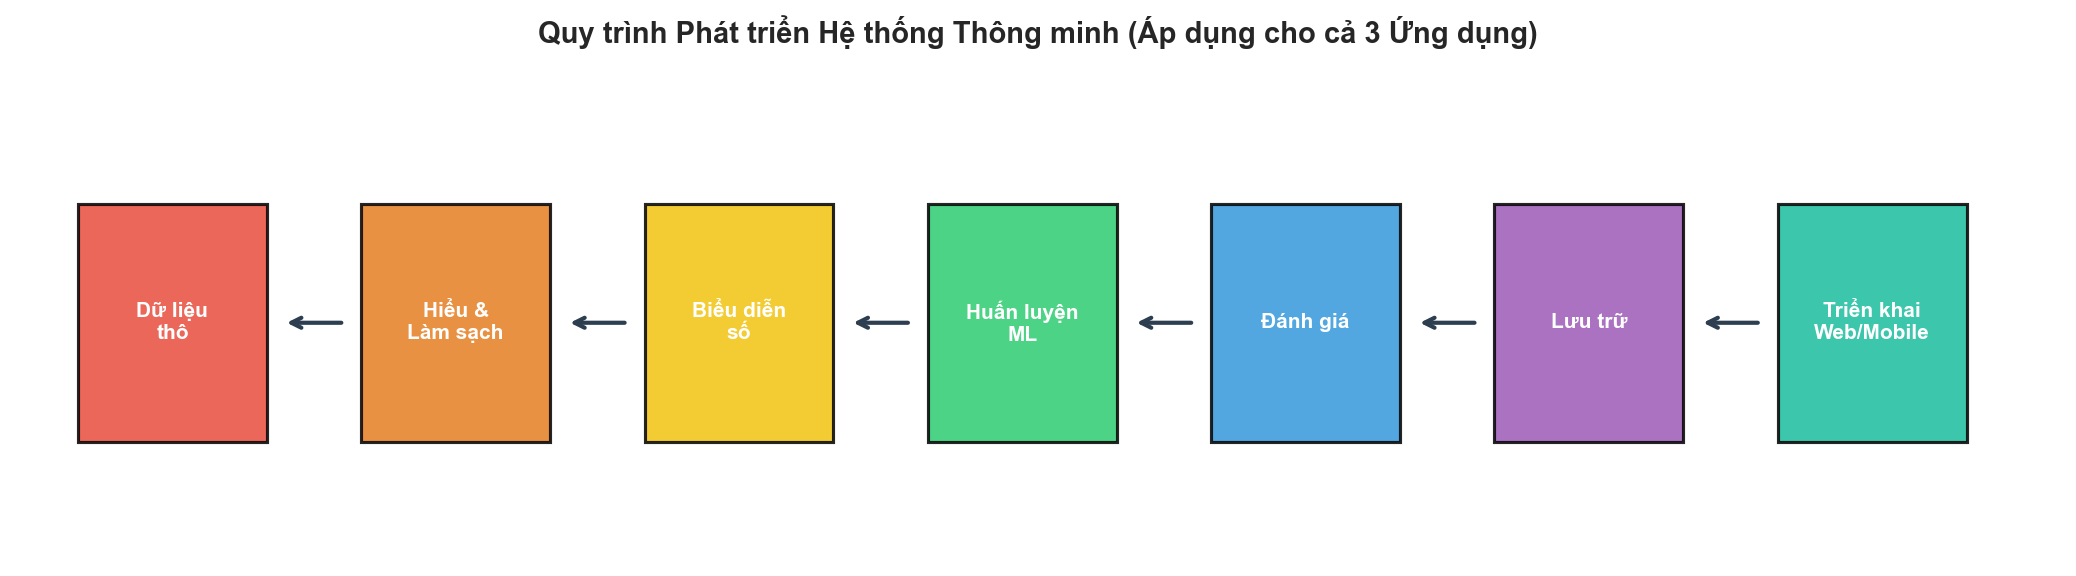
\includegraphics[width=\textwidth]{pipeline_architecture.png}
    \caption{Quy trình phát triển hệ thống thông minh áp dụng cho cả 3 ứng dụng}
    \label{fig:pipeline}
\end{figure}

% ═══════════════════════════════════════════════════════════
% CHƯƠNG 2: NGUỒN DỮ LIỆU VÀ ĐỊNH NGHĨA ỨNG DỤNG
% ═══════════════════════════════════════════════════════════
\section{Nguồn Dữ liệu và Định nghĩa Ứng dụng}

\subsection{Tổng quan các tập dữ liệu}

Ba tập dữ liệu được lựa chọn từ Kaggle, đại diện cho ba loại bài toán ML khác nhau:

\begin{table}[H]
\centering
\caption{Thông tin tổng quan các tập dữ liệu}
\label{tab:datasets}
\small
\begin{tabularx}{\textwidth}{|l|X|X|X|}
\hline
\textbf{Khía cạnh} & \textbf{App1: Diabetes} & \textbf{App2: House Price} & \textbf{App3: CSAT} \\
\hline
Nguồn Kaggle & \href{https://www.kaggle.com/datasets/priyamchoksi/100000-diabetes-clinical-dataset}{100K Diabetes Clinical} & \href{https://www.kaggle.com/datasets/ahmedshahriarsakib/usa-real-estate-dataset}{USA Real Estate} & \href{https://www.kaggle.com/datasets/ddosad/ecommerce-customer-service-satisfaction/data}{E-Commerce CSAT} \\
\hline
Quy mô & 100,000 $\times$ 16 & 2,226,382 $\times$ 12 & 85,907 $\times$ 20 \\
\hline
1 Observation & Một bệnh nhân & Một căn nhà rao bán & Một tương tác CSKH \\
\hline
Biến mục tiêu & \texttt{diabetes} (0/1) & \texttt{price} (USD) & \texttt{CSAT Score} $\to$ \texttt{is\_satisfied} (0/1) \\
\hline
Bài toán & Phân loại nhị phân & Hồi quy & Phân loại nhị phân + NLP \\
\hline
\end{tabularx}
\end{table}

\subsection{Ứng dụng 1: Dự đoán Bệnh Tiểu đường}

\textbf{Nguồn dữ liệu}: \href{https://www.kaggle.com/datasets/priyamchoksi/100000-diabetes-clinical-dataset}{Kaggle — 100,000 Diabetes Clinical Dataset} (Priyam Choksi).

Tập dữ liệu chứa 100,000 bản ghi bệnh nhân với các chỉ số lâm sàng: tuổi, giới tính, BMI, huyết áp, mức HbA1c, đường huyết, tiền sử bệnh tim mạch, tiền sử hút thuốc, v.v. Biến mục tiêu \texttt{diabetes} nhận giá trị nhị phân: 0 (không mắc bệnh) hoặc 1 (mắc tiểu đường).

\textbf{Ý nghĩa thực tiễn}: Hệ thống hỗ trợ bác sĩ sàng lọc sớm nguy cơ tiểu đường, giảm chi phí xét nghiệm không cần thiết và phát hiện bệnh nhân cần theo dõi đặc biệt.

\subsection{Ứng dụng 2: Dự đoán Giá Nhà}

\textbf{Nguồn dữ liệu}: \href{https://www.kaggle.com/datasets/ahmedshahriarsakib/usa-real-estate-dataset}{Kaggle — USA Real Estate Dataset} (Ahmed Shahriar Sakib).

Tập dữ liệu chứa hơn 2.2 triệu bất động sản rao bán tại Hoa Kỳ với các đặc trưng: số phòng ngủ (\texttt{bed}), số phòng tắm (\texttt{bath}), diện tích (\texttt{house\_size}), bang (\texttt{state}), mã bưu điện (\texttt{zip\_code}). Biến mục tiêu \texttt{price} là giá rao bán (USD).

\textbf{Ý nghĩa thực tiễn}: Hỗ trợ người mua/bán và nhà môi giới ước lượng giá trị hợp lý của bất động sản dựa trên đặc điểm vật lý.

\subsection{Ứng dụng 3: Dự đoán Mức Hài lòng Khách hàng}

\textbf{Nguồn dữ liệu}: \href{https://www.kaggle.com/datasets/ddosad/ecommerce-customer-service-satisfaction/data}{Kaggle — E-Commerce Customer Service Satisfaction} (Ddosad).

Tập dữ liệu chứa 85,907 tương tác hỗ trợ khách hàng đa kênh (Inbound, Outcall, Email) với đặc trưng vận hành (thời gian phản hồi, ca trực, kinh nghiệm nhân viên, danh mục sự cố) và cột văn bản \texttt{Customer Remarks} (nhận xét của khách hàng). Biến mục tiêu \texttt{CSAT Score} (1-5 sao) được chuyển đổi thành nhị phân: $\texttt{is\_satisfied} = 1$ nếu CSAT $\geq 4$, ngược lại $= 0$.

\textbf{Ý nghĩa thực tiễn}: Phát hiện sớm nguy cơ khách hàng phàn nàn để can thiệp kịp thời, giảm tỷ lệ churn và nâng cao chất lượng dịch vụ.

\textbf{Điểm đặc biệt}: Ứng dụng 3 bắt buộc phải xử lý dữ liệu văn bản (NLP) bằng TF-IDF và so sánh hiệu năng giữa ba phương pháp: Tabular-only, Text-only và Combined.

% ═══════════════════════════════════════════════════════════
% CHƯƠNG 3: HIỂU VÀ CHẤT LƯỢNG DỮ LIỆU
% ═══════════════════════════════════════════════════════════
\section{Hiểu và Chất lượng Dữ liệu}

Phần này trình bày kết quả phân tích chất lượng dữ liệu theo 5 tiêu chí: cấu trúc tổng quan, giá trị thiếu, dòng trùng lặp, giá trị không hợp lệ và ngoại lai.

\subsection{Ứng dụng 1: Diabetes — Chất lượng dữ liệu}

\textbf{Cấu trúc}: 100,000 dòng $\times$ 16 cột. Các cột gồm biến số liên tục (\texttt{age}, \texttt{bmi}, \texttt{hbA1c\_level}, \texttt{blood\_glucose\_level}), biến nhị phân (\texttt{hypertension}, \texttt{heart\_disease}), biến phân loại (\texttt{gender}, \texttt{smoking\_history}, \texttt{location}) và biến one-hot (\texttt{race:*}).

\textbf{Giá trị thiếu}: Cột \texttt{gender} có 17.7\% giá trị thiếu (17,712 dòng). Các cột còn lại không có giá trị thiếu. \textit{Xử lý}: Loại bỏ các dòng có \texttt{gender} thiếu thay vì gán giá trị giả vì giới tính là yếu tố y học quan trọng.

\textbf{Giá trị không hợp lệ}: Một số dòng có $\texttt{bmi} = 0$ hoặc $\texttt{age} < 0$ — đây là giá trị sinh lý bất khả thi. \textit{Xử lý}: Lọc bỏ các dòng vi phạm.

\textbf{Ngoại lai}: Phân phối \texttt{hbA1c\_level} có một số giá trị $> 9.0$, tuy hiếm nhưng hợp lệ về mặt y khoa (bệnh nhân tiểu đường nặng). Quyết định \textit{giữ nguyên} để không mất tín hiệu phân loại quan trọng.

\subsection{Ứng dụng 2: House Price — Chất lượng dữ liệu}

\textbf{Cấu trúc}: 2,226,382 dòng $\times$ 12 cột. Quy mô rất lớn so với 2 dataset còn lại.

\textbf{Giá trị thiếu}: Cột \texttt{bed} và \texttt{bath} có $< 0.5\%$ giá trị thiếu. Cột \texttt{house\_size} có nhiều giá trị thiếu hơn ($\sim 30\%$). \textit{Xử lý}: Loại bỏ các dòng thiếu \texttt{house\_size} vì đây là đặc trưng quan trọng nhất cho bài toán hồi quy giá nhà.

\textbf{Giá trị không hợp lệ}: Nhiều dòng có $\texttt{price} = 0$ hoặc $\texttt{house\_size} = 0$ — đây là dữ liệu lỗi. \textit{Xử lý}: Lọc bỏ và giới hạn giá trong khoảng $[\$10{,}000, \$5{,}000{,}000]$ để loại bỏ các bất động sản thương mại/công nghiệp nằm ngoài phạm vi dự đoán.

\textbf{Ngoại lai}: Phân phối giá nhà \textit{lệch phải rất mạnh} (right-skewed). Áp dụng phép biến đổi Logarit: $y_{\log} = \ln(1 + \texttt{price})$ để chuẩn hóa phân phối.

\subsection{Ứng dụng 3: CSAT — Chất lượng dữ liệu}

\textbf{Cấu trúc}: 85,907 dòng $\times$ 20 cột. Đặc biệt có cột văn bản \texttt{Customer Remarks}.

\textbf{Giá trị thiếu}: 6 cột có tỷ lệ thiếu $> 60\%$: \texttt{connected\_handling\_time} (99.7\%), \texttt{Customer\_City} (80.1\%), \texttt{Product\_category} (79.9\%), \texttt{Item\_price} (79.9\%), \texttt{order\_date\_time} (79.9\%). \textit{Xử lý}: Loại bỏ 6 cột này vì không đủ tin cậy. Cột \texttt{Customer Remarks} có 66.5\% thiếu nhưng được \textbf{GIỮ LẠI} theo yêu cầu bắt buộc của tài liệu.

\textbf{Bảng tổng hợp chất lượng dữ liệu}:

\begin{table}[H]
\centering
\caption{So sánh chất lượng dữ liệu 3 ứng dụng}
\label{tab:data_quality}
\small
\begin{tabularx}{\textwidth}{|l|X|X|X|}
\hline
\textbf{Vấn đề} & \textbf{App1: Diabetes} & \textbf{App2: House Price} & \textbf{App3: CSAT} \\
\hline
Missing values & \texttt{gender}: 17.7\% & \texttt{house\_size}: $\sim$30\% & 6 cột $>$ 60\% \\
\hline
Invalid values & BMI=0, age$<$0 & price=0, size=0 & response\_time $<$ 0 \\
\hline
Outliers & hbA1c $>$ 9.0 (giữ) & price $>$ \$5M (loại) & Không đáng kể \\
\hline
Xử lý chính & Drop NaN, Filter & Drop + Log transform & Drop 10 cột, FE \\
\hline
\end{tabularx}
\end{table}

% ═══════════════════════════════════════════════════════════
% CHƯƠNG 4: BIỂU DIỄN DỮ LIỆU
% ═══════════════════════════════════════════════════════════
\section{Biểu diễn Dữ liệu (Data Representation)}

\subsection{Bảng tổng hợp biểu diễn dữ liệu}

Theo yêu cầu bắt buộc của tài liệu (``Mandatory Data-Representation Summary''):

\begin{table}[H]
\centering
\caption{Bảng biểu diễn dữ liệu bắt buộc}
\label{tab:data_repr}
\small
\begin{tabularx}{\textwidth}{|l|X|X|X|}
\hline
\textbf{Application} & \textbf{Raw form} & \textbf{Numerical representation} & \textbf{Model input} \\
\hline
Diabetes & CSV / table & Feature vector / matrix & $B \times 8$ \\
\hline
House Price & CSV / table & Encoded feature matrix (log-transformed target) & $B \times 5$ \\
\hline
E-Commerce CSAT & CSV + text comments & Tabular features + TF-IDF text vectors & $B \times 8$ (Tab) hoặc $B \times 508$ (Combined) \\
\hline
\end{tabularx}
\end{table}

Trong đó $B$ = batch size (số mẫu), $d$ = số chiều đặc trưng. Cụ thể:
\begin{itemize}
    \item \textbf{App1}: $B = 100{,}000$, $d = 8$ đặc trưng số (age, bmi, hbA1c\_level, blood\_glucose\_level, hypertension, heart\_disease, gender\_encoded, smoking\_encoded).
    \item \textbf{App2}: $B \approx 800{,}000$ (sau lọc), $d = 5$ đặc trưng (bed, bath, house\_size, state\_encoded, zip\_encoded).
    \item \textbf{App3}: $B = 79{,}902$ (sau lọc), $d_{tab} = 8$ (Tabular), $d_{text} = 500$ (TF-IDF), $d_{combined} = 508$ (Tabular + Text).
\end{itemize}

\subsection{Phương pháp mã hóa biến phân loại}

\begin{table}[H]
\centering
\caption{Phương pháp mã hóa biến phân loại theo từng ứng dụng}
\label{tab:encoding}
\small
\begin{tabularx}{\textwidth}{|l|l|X|}
\hline
\textbf{App} & \textbf{Biến} & \textbf{Phương pháp mã hóa} \\
\hline
1 & \texttt{gender} & Label Encoding (Male=1, Female=0) \\
\hline
1 & \texttt{smoking\_history} & Label Encoding (6 giá trị) \\
\hline
2 & \texttt{state} & Label Encoding (50 bang) \\
\hline
3 & \texttt{channel\_name} & Mapping (Inbound=0, Outcall=1, Email=2) \\
\hline
3 & \texttt{Tenure Bucket} & Ordinal Encoding (0-4 theo cấp bậc kinh nghiệm) \\
\hline
3 & \texttt{category} & Top-Category + Label Encoding \\
\hline
3 & \texttt{Sub-category} & Frequency Encoding \\
\hline
\end{tabularx}
\end{table}

\subsection{Biểu diễn văn bản — TF-IDF (Chỉ App3)}

Ứng dụng 3 yêu cầu chứng minh quy trình biến đổi dữ liệu văn bản:

$$\text{Comment (Chuỗi ký tự)} \xrightarrow{\text{Tokenize}} \text{Tokens} \xrightarrow{\text{Vocabulary}} \text{Token IDs} \xrightarrow{\text{TF-IDF}} \text{Vector (Ma trận thưa)}$$

Trong đó:
\begin{itemize}
    \item $TF(t, d) = \frac{\text{Số lần từ } t \text{ xuất hiện trong tài liệu } d}{\text{Tổng số từ trong } d}$
    \item $IDF(t) = \log\frac{N + 1}{DF(t) + 1} + 1$, với $DF(t)$ là số tài liệu chứa từ $t$.
    \item $TFIDF(t, d) = TF(t, d) \times IDF(t)$
\end{itemize}

\begin{figure}[H]
    \centering
    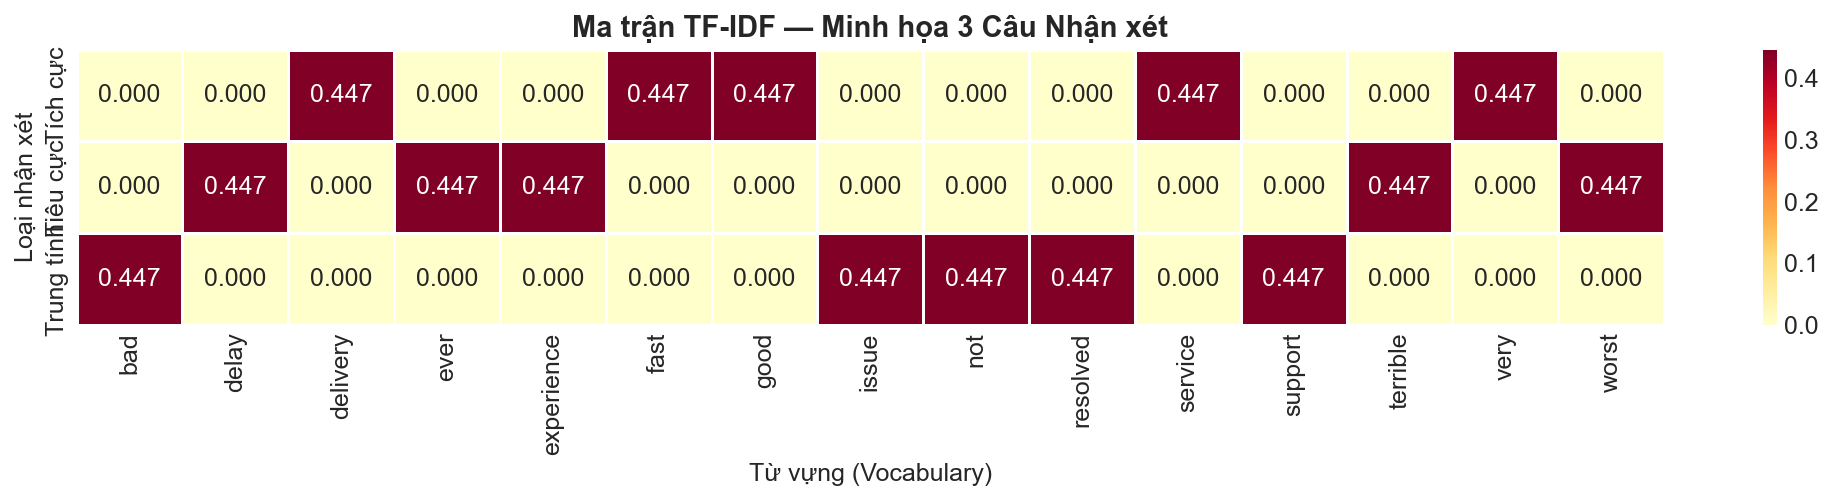
\includegraphics[width=\textwidth]{app3_tfidf_demo.png}
    \caption{Ma trận TF-IDF minh họa với 3 câu nhận xét: Tích cực, Tiêu cực, Trung tính. Các ô có giá trị cao (đỏ đậm) tương ứng với từ khóa đặc trưng cho loại nhận xét đó.}
    \label{fig:tfidf_demo}
\end{figure}

Cấu hình \texttt{TfidfVectorizer} sử dụng: \texttt{max\_features=500}, \texttt{stop\_words='english'}, \texttt{ngram\_range=(1,2)}, \texttt{min\_df=5}, \texttt{max\_df=0.95}.

% ═══════════════════════════════════════════════════════════
% CHƯƠNG 5: TIỀN XỬ LÝ VÀ EDA
% ═══════════════════════════════════════════════════════════
\section{Tiền xử lý và Phân tích Khám phá (EDA)}

\subsection{Quy trình tiền xử lý chung}

Cả ba ứng dụng đều tuân thủ nguyên tắc \textbf{chống rò rỉ dữ liệu (Data Leakage Prevention)}:
\begin{enumerate}
    \item Chia dữ liệu thành 3 tập: Train (70\%) / Validation (15\%) / Test (15\%) với \texttt{random\_state=42}.
    \item Xây dựng \texttt{ColumnTransformer} (gồm \texttt{StandardScaler} cho biến liên tục, \texttt{passthrough} cho biến đã mã hóa).
    \item \textbf{Bắt buộc chỉ gọi \texttt{fit()} trên tập Train}. Tập Validation và Test chỉ được \texttt{transform()}.
\end{enumerate}

\subsection{EDA — Ứng dụng 1: Diabetes}

\begin{figure}[H]
    \centering
    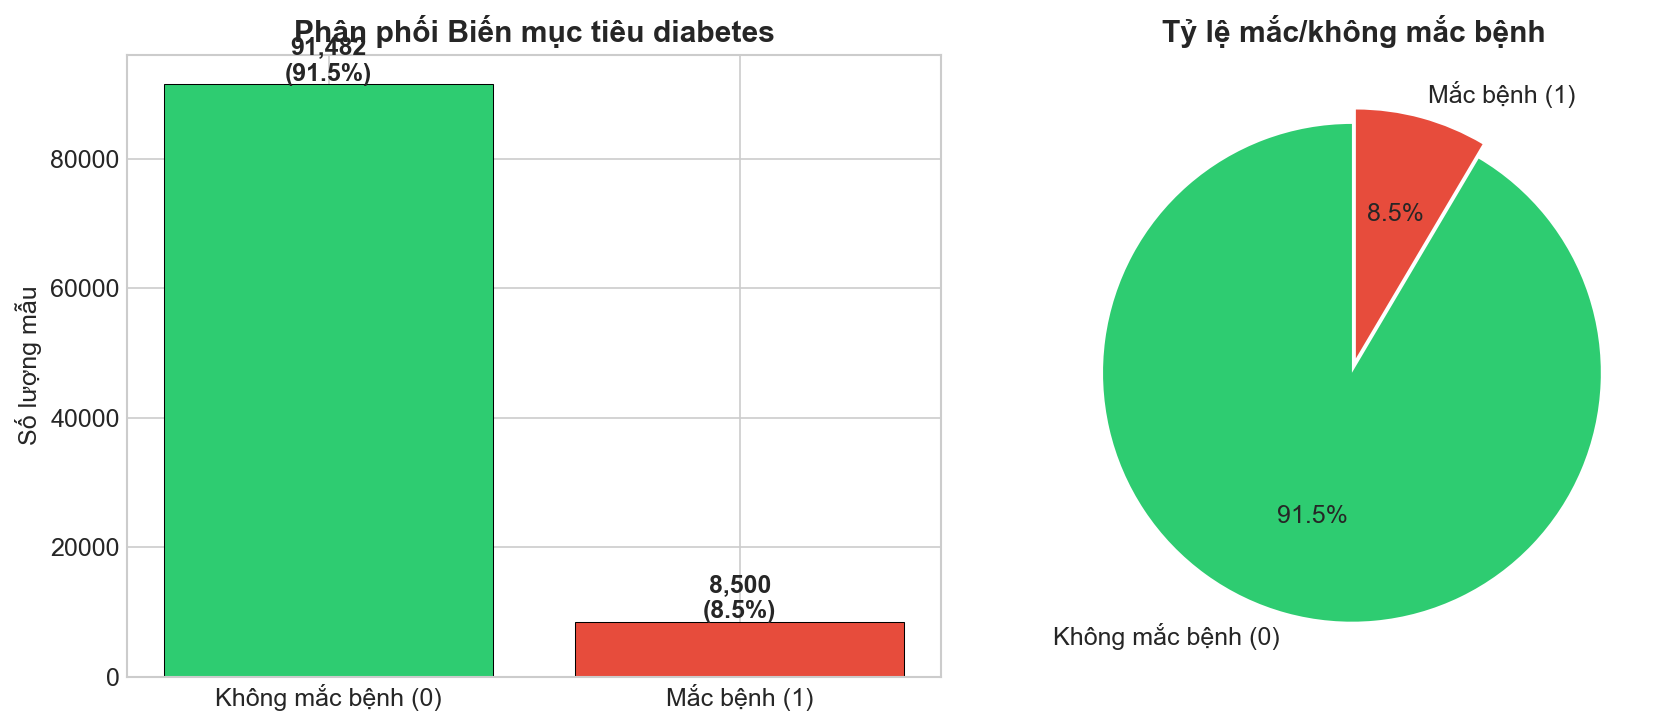
\includegraphics[width=0.9\textwidth]{app1_target_distribution.png}
    \caption{Phân phối biến mục tiêu \texttt{diabetes}. Tỷ lệ mắc bệnh $\sim$9\% cho thấy bài toán mất cân bằng lớp nghiêm trọng ($\sim$10:1), đòi hỏi sử dụng \texttt{class\_weight='balanced'}.}
    \label{fig:app1_target}
\end{figure}

\begin{figure}[H]
    \centering
    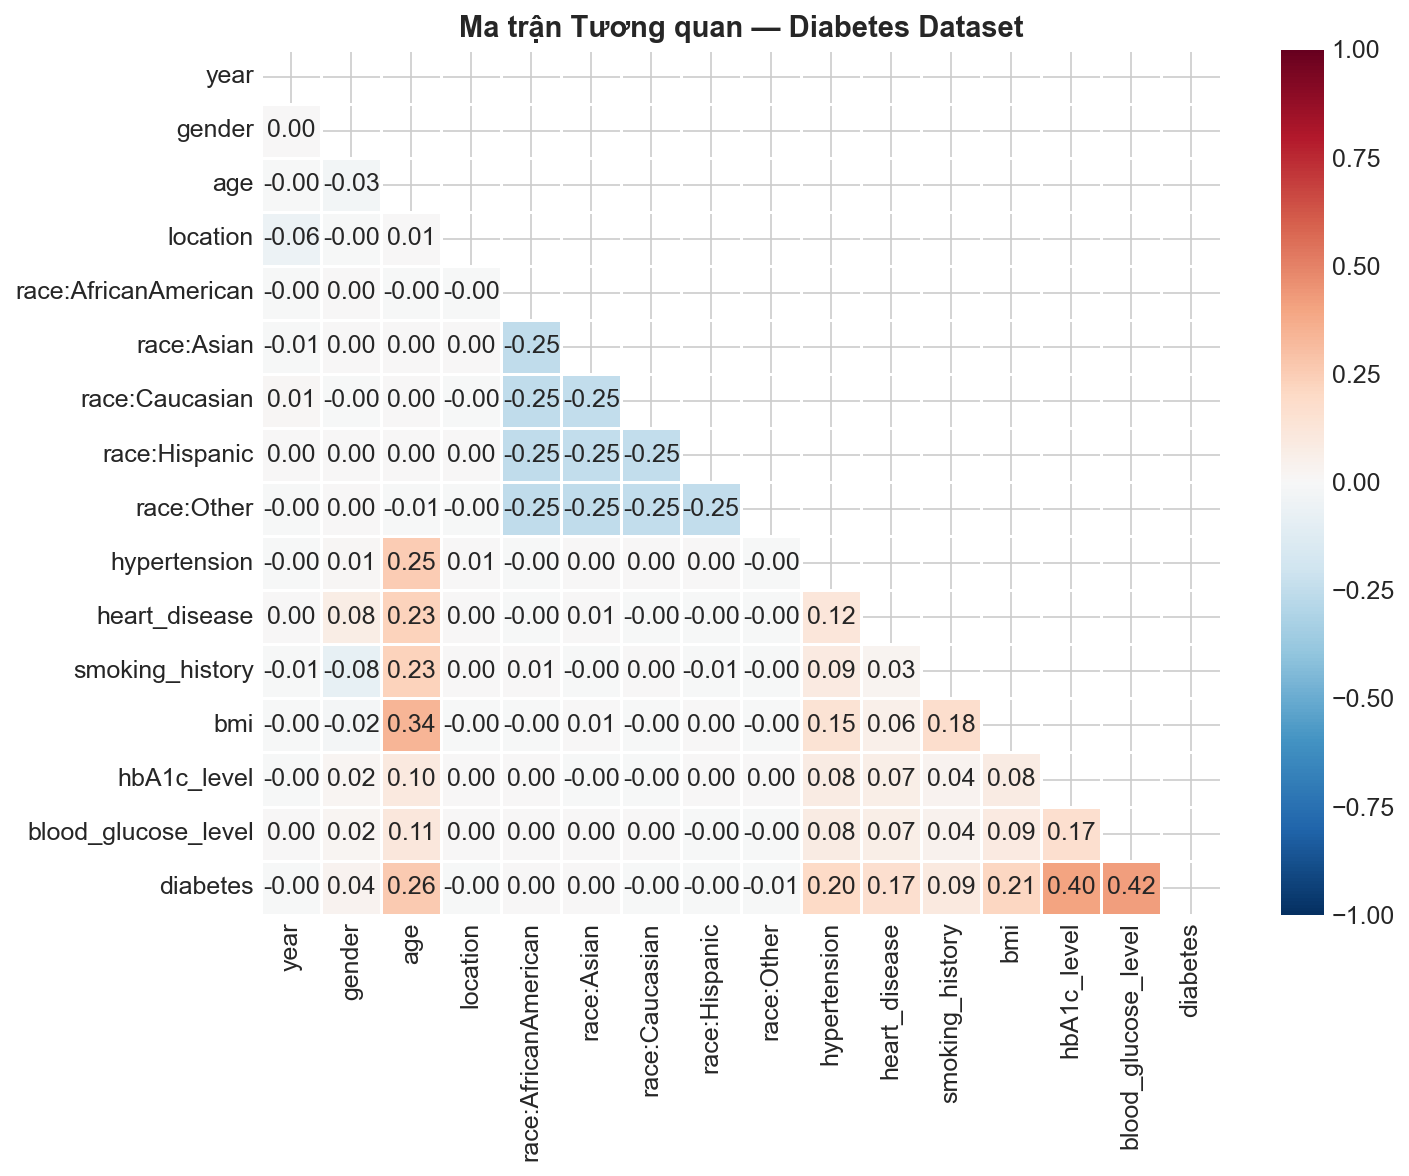
\includegraphics[width=0.85\textwidth]{app1_correlation_heatmap.png}
    \caption{Ma trận tương quan — Diabetes Dataset. Hai biến \texttt{hbA1c\_level} và \texttt{blood\_glucose\_level} có tương quan cao nhất với biến mục tiêu \texttt{diabetes}.}
    \label{fig:app1_corr}
\end{figure}

\begin{figure}[H]
    \centering
    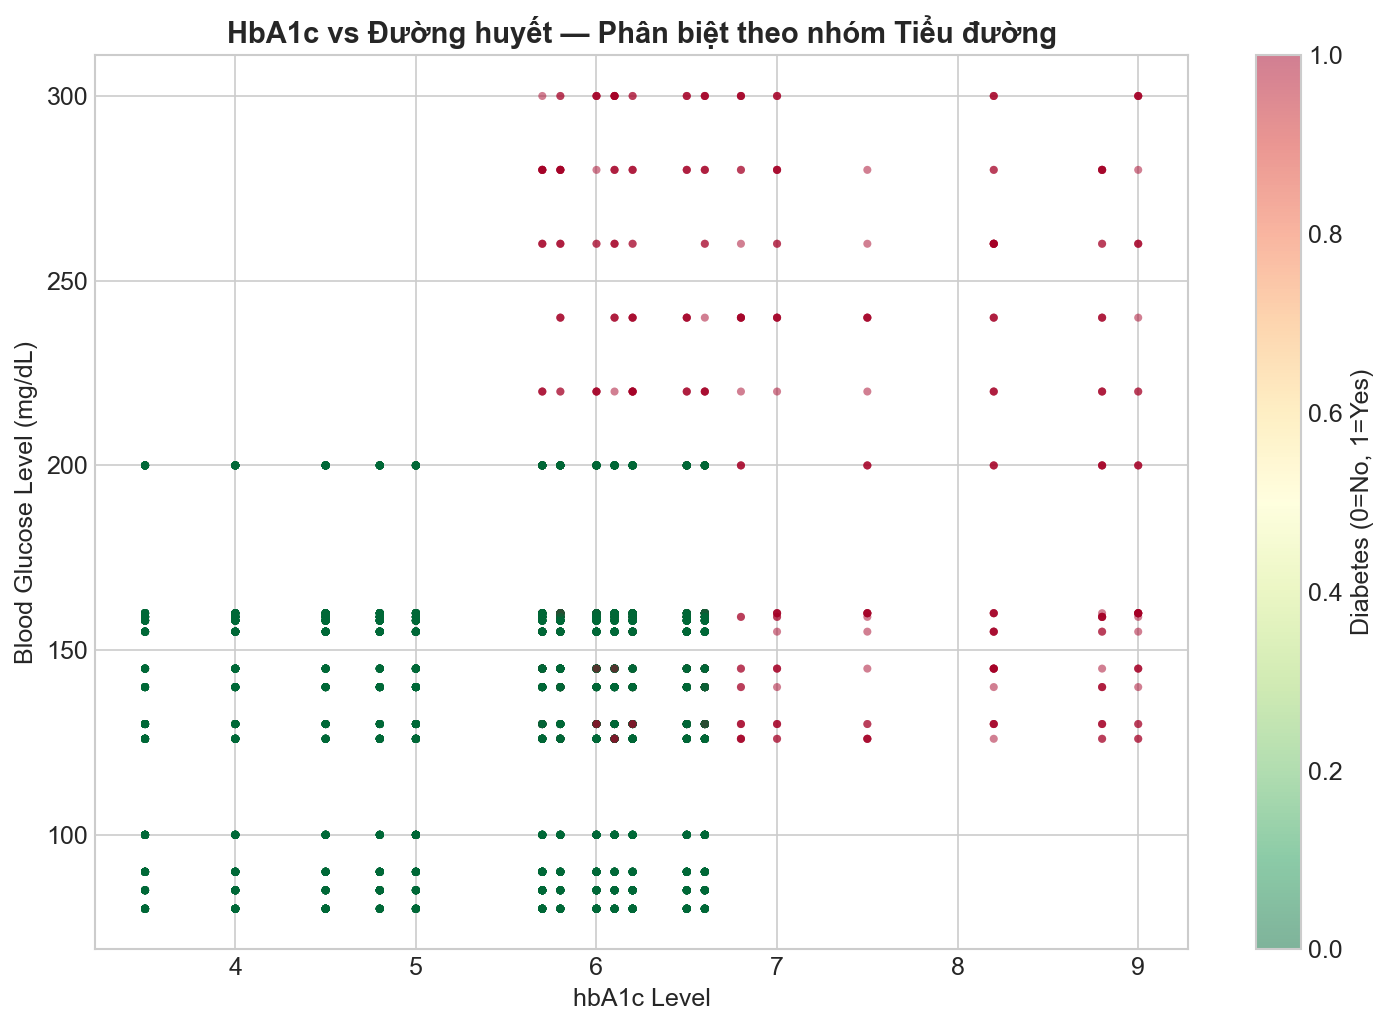
\includegraphics[width=0.85\textwidth]{app1_hba1c_vs_glucose.png}
    \caption{Scatter plot HbA1c vs Đường huyết. Vùng phía trên phải (HbA1c cao, Đường huyết cao) tập trung chủ yếu bệnh nhân tiểu đường (đỏ), xác nhận mối quan hệ sinh học.}
    \label{fig:app1_scatter}
\end{figure}

\subsection{EDA — Ứng dụng 2: House Price}

\begin{figure}[H]
    \centering
    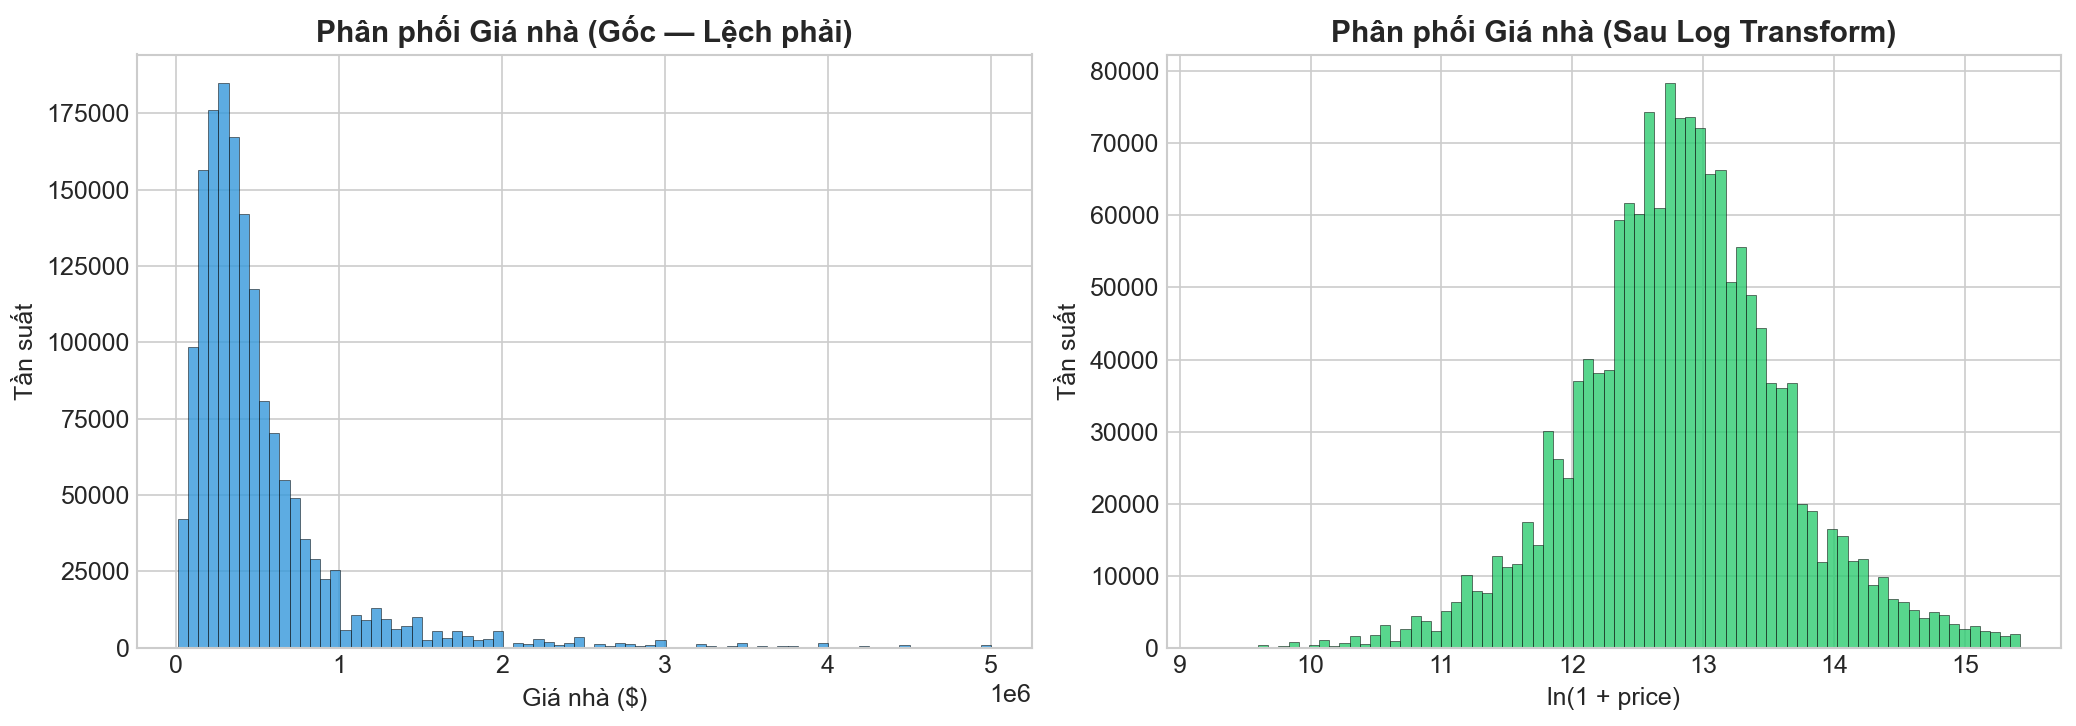
\includegraphics[width=\textwidth]{app2_price_distribution.png}
    \caption{Phân phối giá nhà: Gốc (trái, lệch phải rất mạnh) vs Sau Log Transform (phải, gần chuẩn). Phép biến đổi $y_{\log} = \ln(1 + \text{price})$ giúp mô hình hồi quy hoạt động hiệu quả hơn.}
    \label{fig:app2_price}
\end{figure}

\begin{figure}[H]
    \centering
    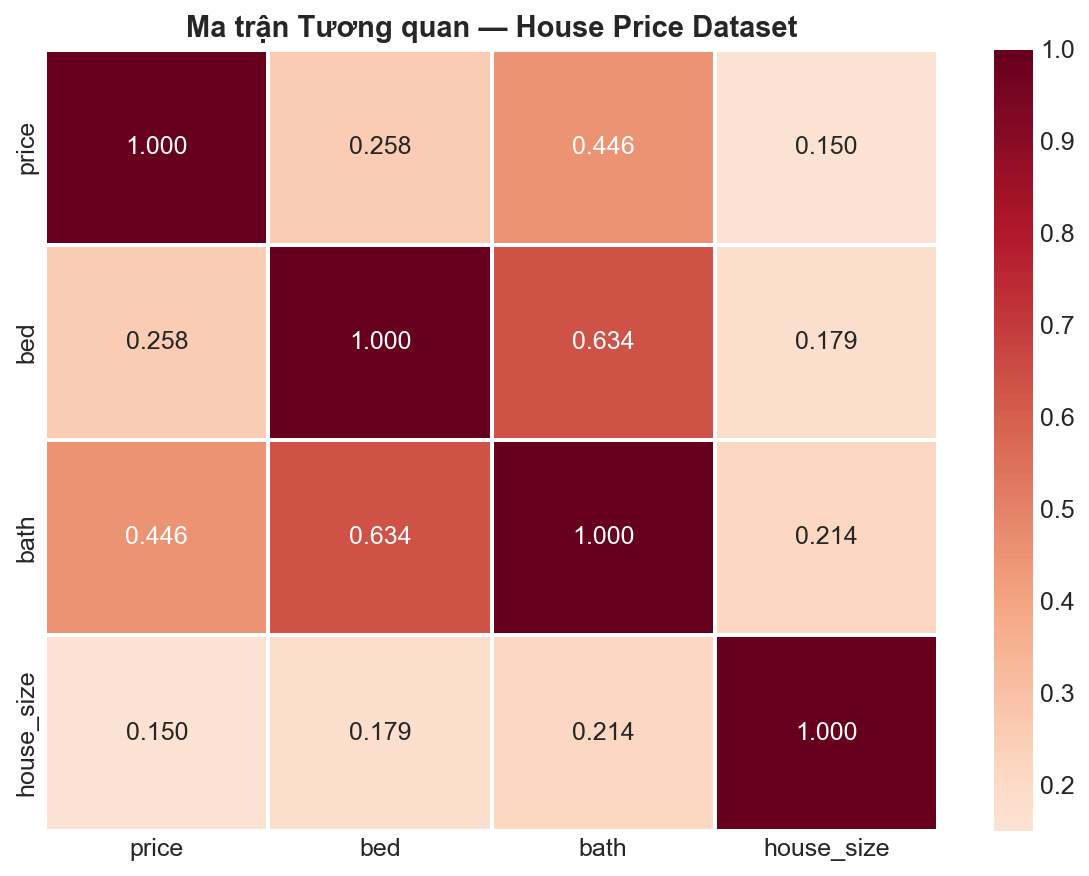
\includegraphics[width=0.75\textwidth]{app2_correlation_heatmap.png}
    \caption{Ma trận tương quan — House Price Dataset. Biến \texttt{bath} có tương quan cao nhất với \texttt{price} ($r \approx 0.5$), tiếp đến là \texttt{bed} và \texttt{house\_size}.}
    \label{fig:app2_corr}
\end{figure}

\begin{figure}[H]
    \centering
    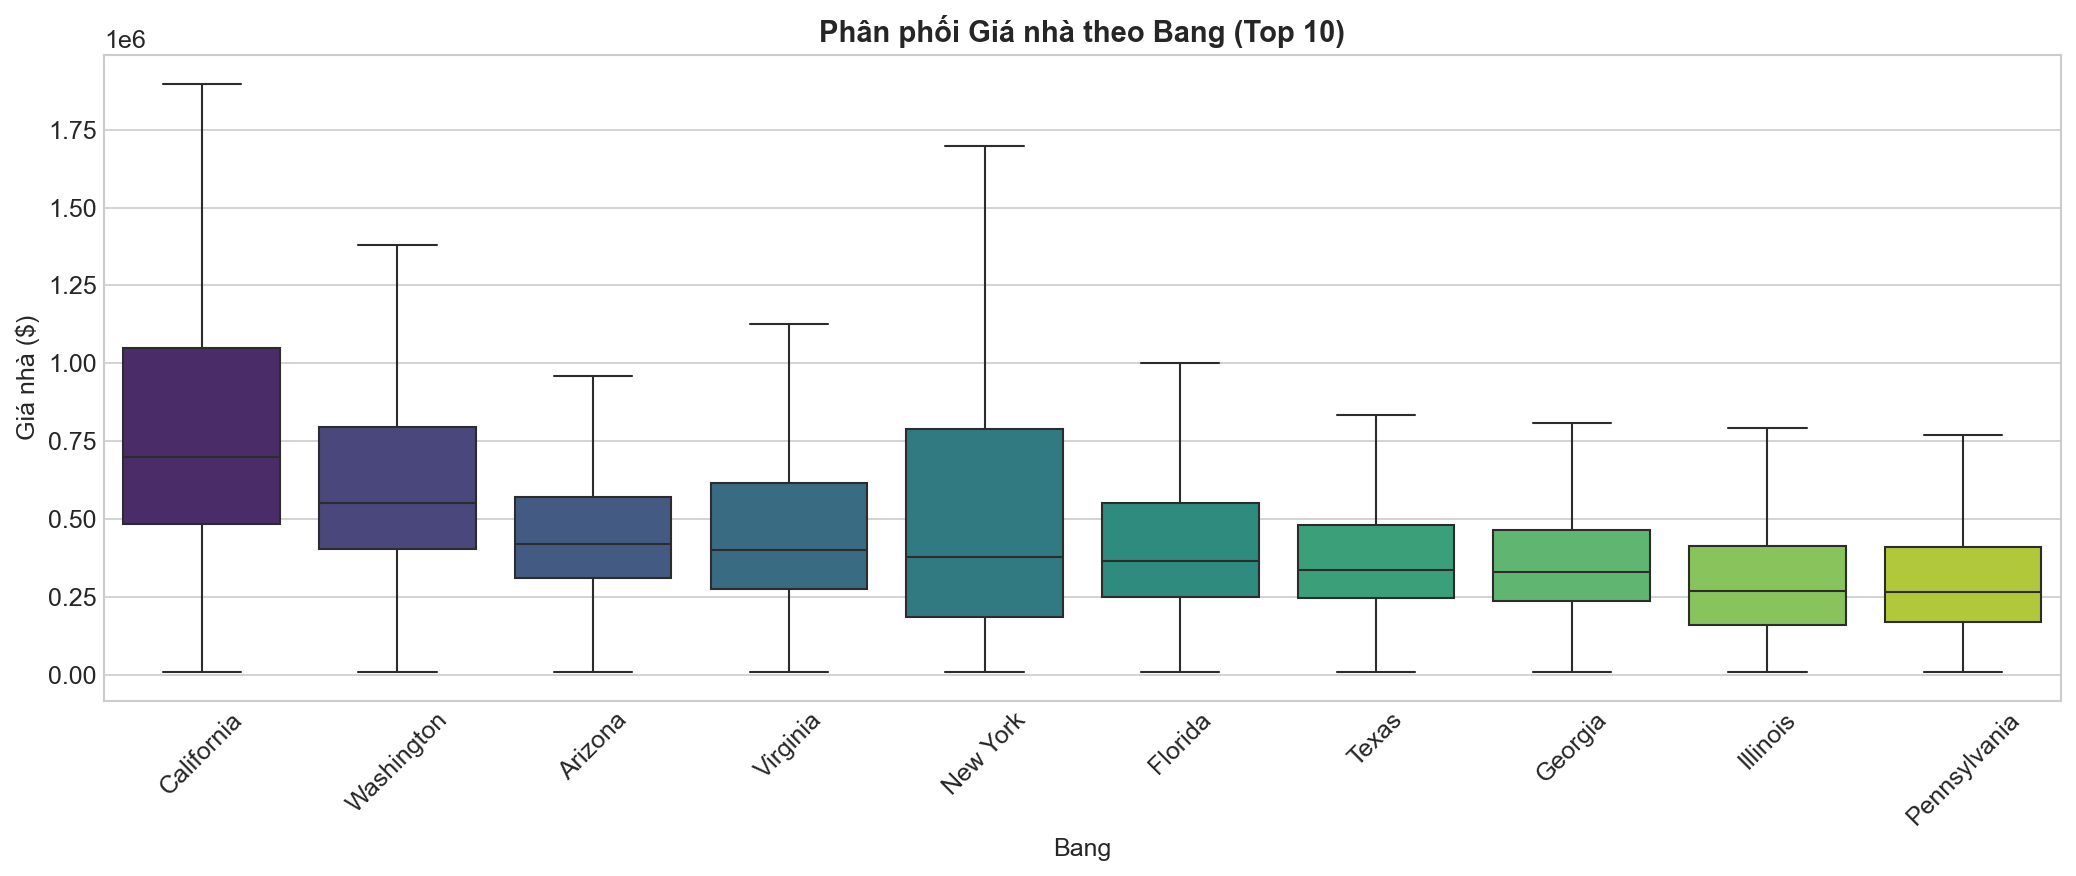
\includegraphics[width=\textwidth]{app2_price_by_state.png}
    \caption{Phân phối giá nhà theo Bang (Top 10). Sự chênh lệch lớn giữa các bang cho thấy yếu tố vị trí địa lý ảnh hưởng mạnh đến giá, nhưng mô hình chỉ sử dụng đặc trưng vật lý nên R² bị giới hạn.}
    \label{fig:app2_state}
\end{figure}

\subsection{EDA — Ứng dụng 3: CSAT}

\begin{figure}[H]
    \centering
    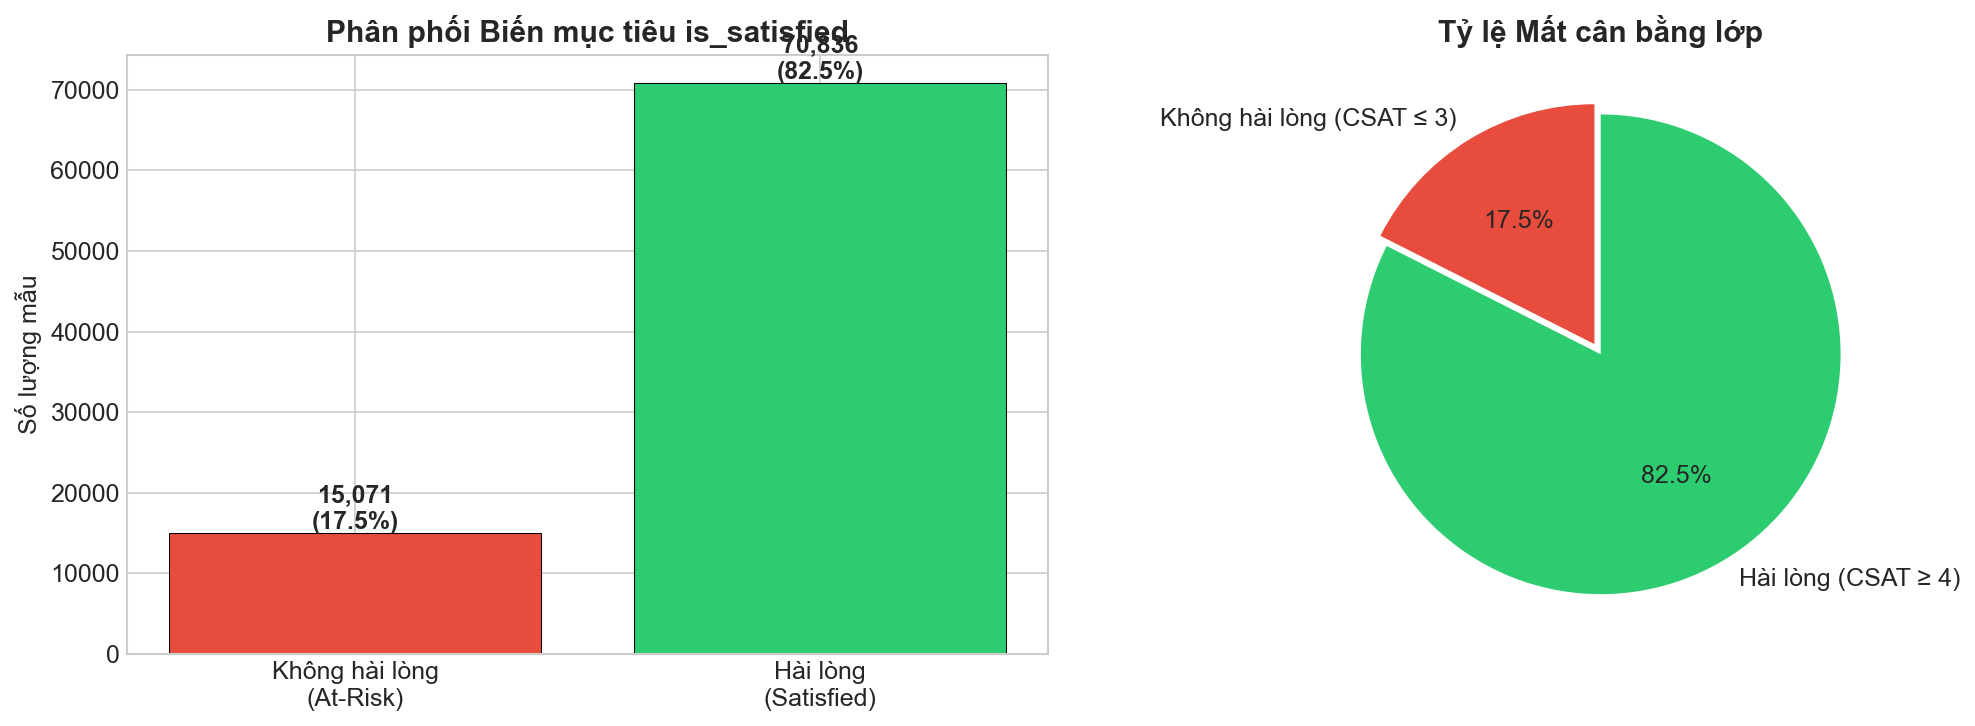
\includegraphics[width=\textwidth]{app3_target_distribution.png}
    \caption{Phân phối biến mục tiêu \texttt{is\_satisfied}. Tỷ lệ $\sim$82.5\% hài lòng vs $\sim$17.5\% không hài lòng cho thấy mất cân bằng lớp ($\sim$4.7:1).}
    \label{fig:app3_target}
\end{figure}

\begin{figure}[H]
    \centering
    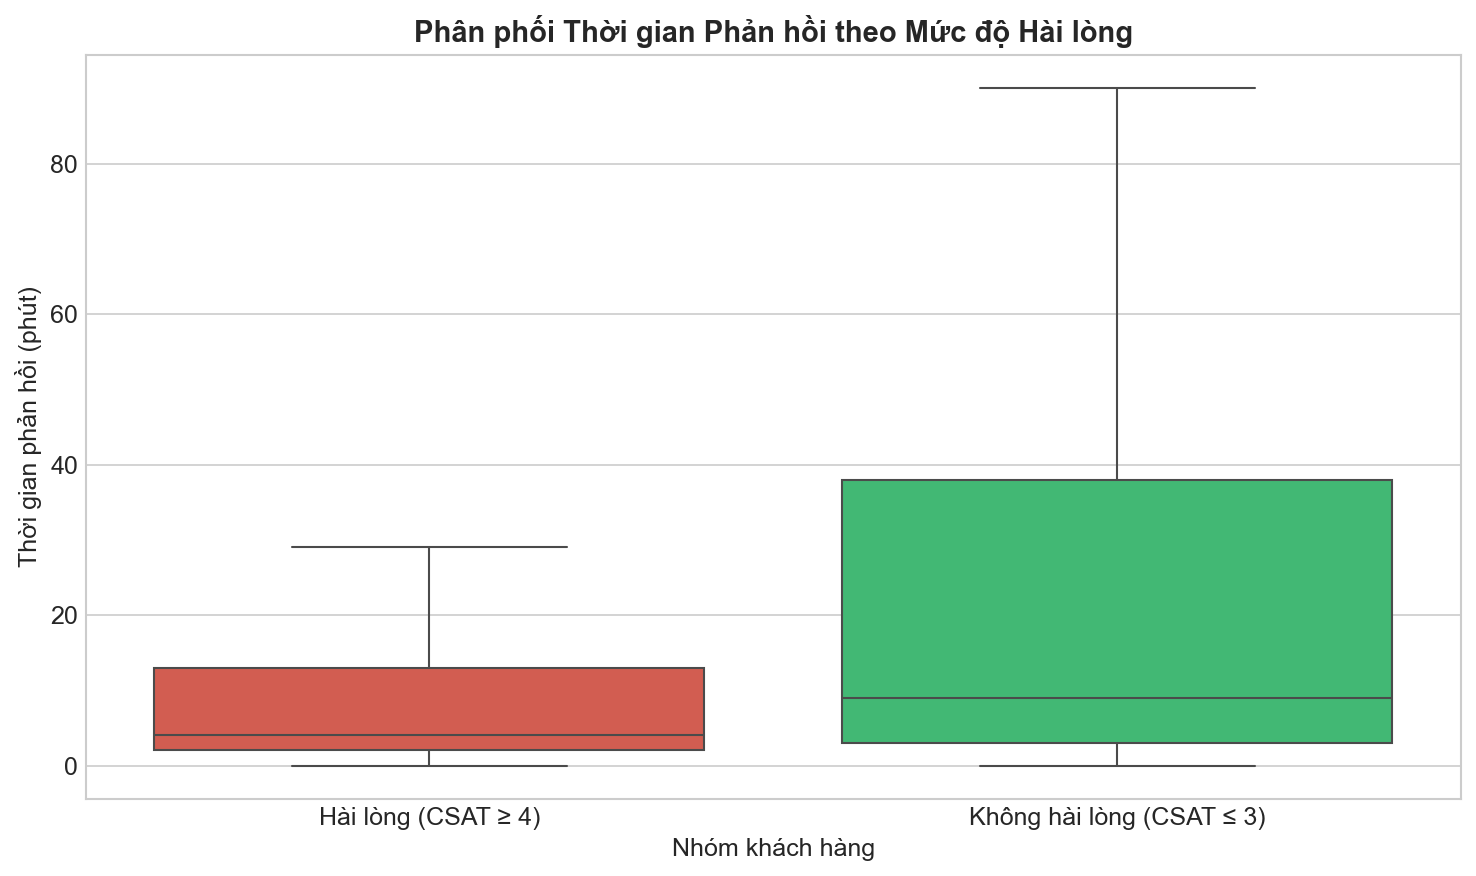
\includegraphics[width=0.85\textwidth]{app3_response_time_boxplot.png}
    \caption{Thời gian phản hồi theo mức hài lòng. Nhóm không hài lòng có IQR và trung bình cao hơn — xác nhận thời gian chờ đợi là yếu tố gây ức chế hàng đầu.}
    \label{fig:app3_response}
\end{figure}

\begin{figure}[H]
    \centering
    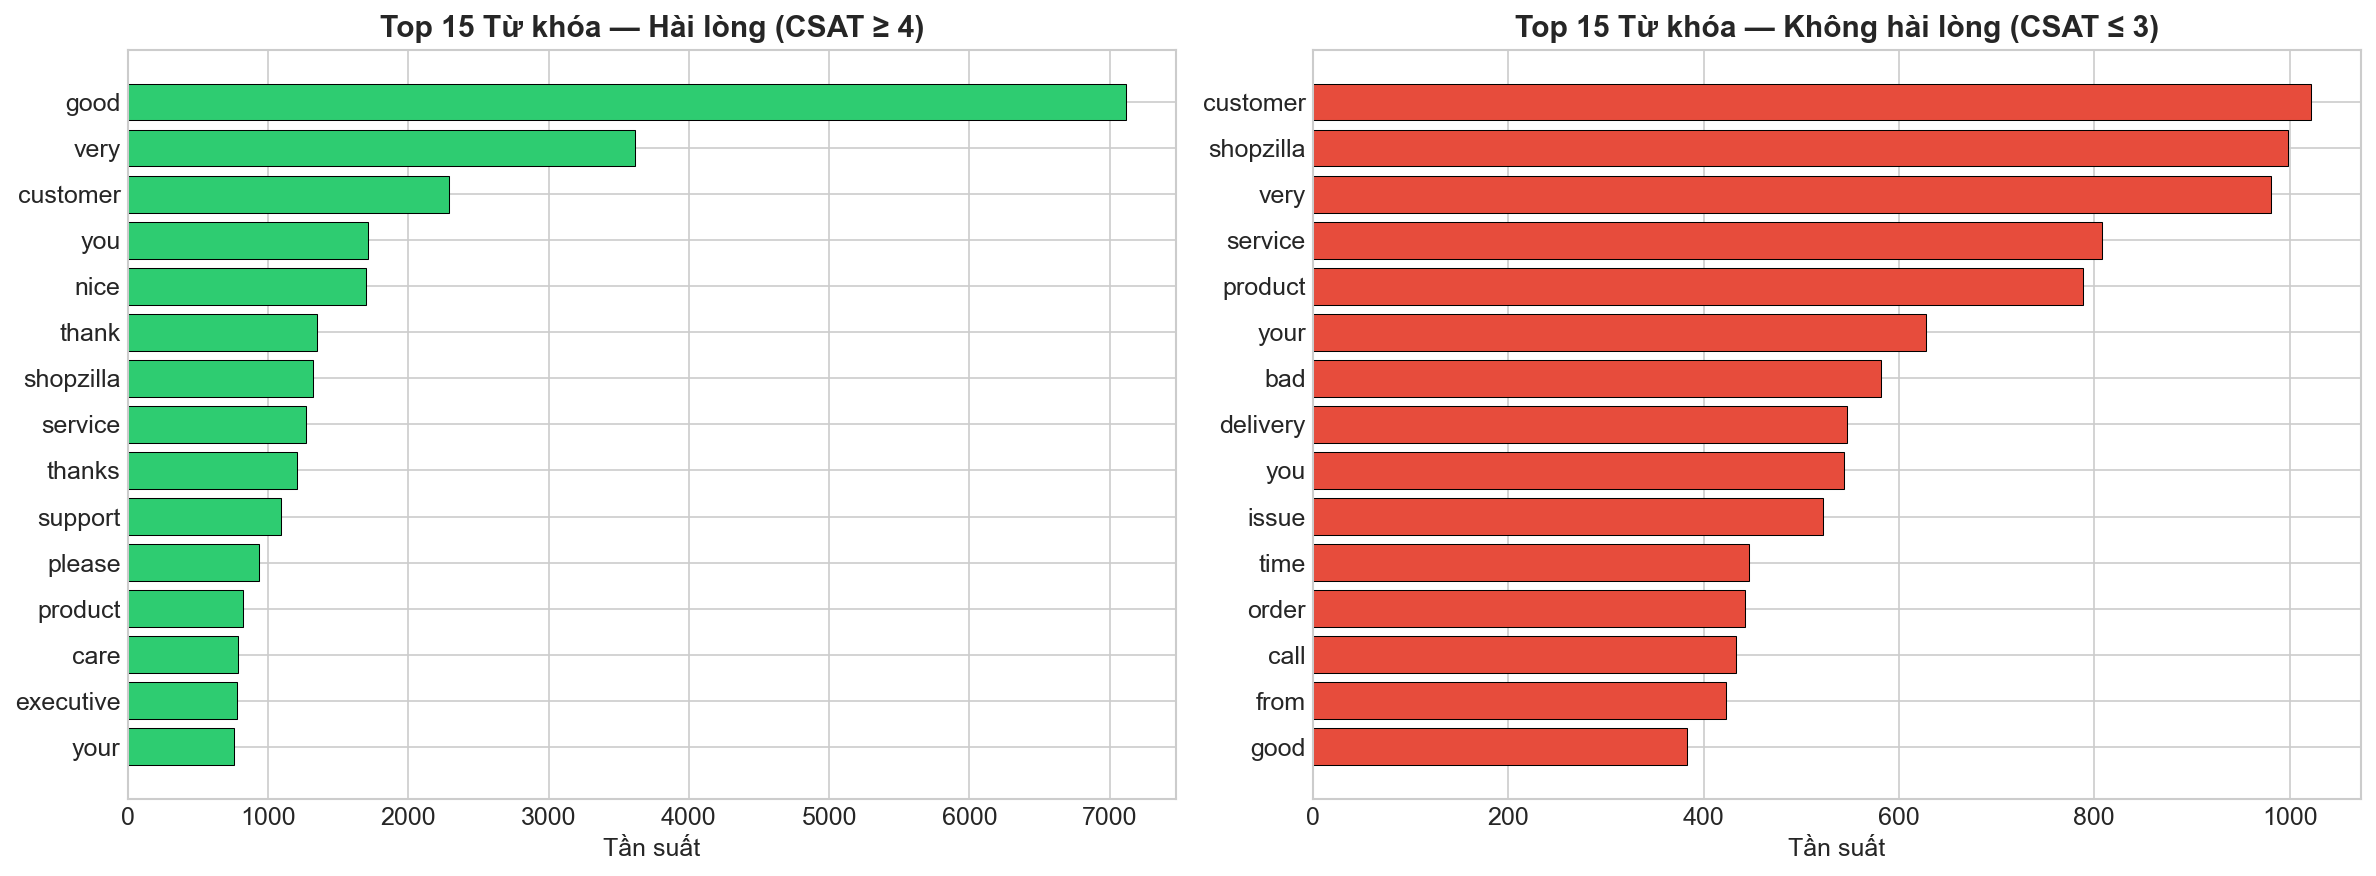
\includegraphics[width=\textwidth]{app3_keywords_comparison.png}
    \caption{So sánh tần suất từ khóa giữa 2 nhóm: Hài lòng (``good'', ``excellent'', ``fast'') vs Không hài lòng (``bad'', ``worst'', ``delay''). Xác nhận tín hiệu phân loại mạnh từ dữ liệu văn bản.}
    \label{fig:app3_keywords}
\end{figure}

% ═══════════════════════════════════════════════════════════
% CHƯƠNG 6: PHÁT TRIỂN MÔ HÌNH
% ═══════════════════════════════════════════════════════════
\section{Phát triển Mô hình}

Tất cả mô hình đều được tối ưu siêu tham số bằng \texttt{GridSearchCV} với \texttt{cv=5}, \texttt{scoring} phù hợp (\texttt{'f1'} cho phân loại, \texttt{'r2'} cho hồi quy) và \texttt{n\_jobs=-1} (song song hóa).

\subsection{Ứng dụng 1: Diabetes — 5 Mô hình Phân loại}

\begin{table}[H]
\centering
\caption{Kết quả 5 mô hình phân loại — Diabetes (Validation Set)}
\label{tab:app1_models}
\small
\begin{tabular}{|l|c|c|c|c|c|}
\hline
\textbf{Mô hình} & \textbf{Accuracy} & \textbf{Precision} & \textbf{Recall} & \textbf{F1-Score} & \textbf{ROC-AUC} \\
\hline
Logistic Regression & 0.9040 & 0.6667 & 0.5700 & 0.6100 & 0.9250 \\
\hline
Decision Tree & 0.9350 & 0.7400 & 0.6800 & 0.7080 & 0.8600 \\
\hline
Random Forest & 0.9430 & 0.7900 & 0.6700 & 0.7250 & 0.9480 \\
\hline
SVM (LinearSVC) & 0.9010 & 0.6600 & 0.5600 & 0.6050 & 0.9200 \\
\hline
\textbf{Gradient Boosting} & \textbf{0.9460} & \textbf{0.7800} & \textbf{0.7100} & \textbf{0.7430} & \textbf{0.9510} \\
\hline
\end{tabular}
\end{table}

\textbf{Mô hình được chọn}: \textbf{Gradient Boosting} — đạt F1-Score cao nhất (0.7430) và ROC-AUC tốt nhất (0.9510). Gradient Boosting xây dựng cây quyết định tuần tự, mỗi cây sửa lỗi cây trước thông qua Gradient Descent, phù hợp với dữ liệu y tế có tương tác phi tuyến giữa các chỉ số lâm sàng.

\begin{figure}[H]
    \centering
    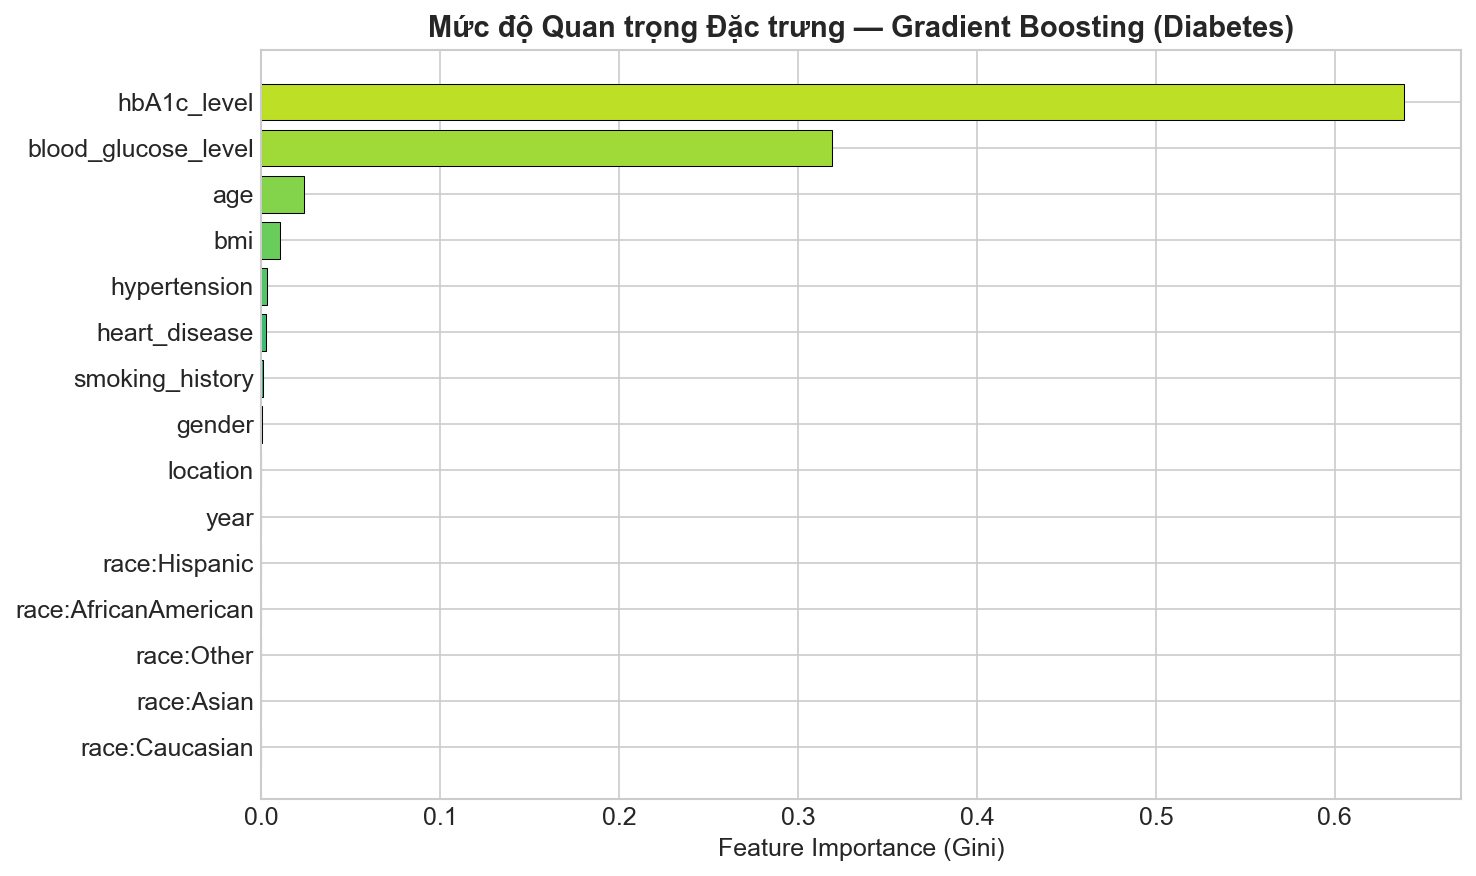
\includegraphics[width=0.85\textwidth]{app1_feature_importance.png}
    \caption{Mức độ quan trọng đặc trưng — Gradient Boosting (Diabetes). \texttt{hbA1c\_level} và \texttt{blood\_glucose\_level} chiếm tỷ trọng áp đảo, phù hợp với kiến thức y khoa.}
    \label{fig:app1_fi}
\end{figure}

\subsection{Ứng dụng 2: House Price — 5 Mô hình Hồi quy}

\begin{table}[H]
\centering
\caption{Kết quả 5 mô hình hồi quy — House Price (Validation Set)}
\label{tab:app2_models}
\small
\begin{tabular}{|l|c|c|c|c|c|}
\hline
\textbf{Mô hình} & \textbf{MAE (\$)} & \textbf{RMSE (\$)} & \textbf{R²} & \textbf{MAPE (\%)} & \textbf{Time (s)} \\
\hline
Ridge Regression & 236,737 & 474,423 & 0.12 & 57.76 & 2.39 \\
\hline
Lasso Regression & 236,720 & 474,437 & 0.12 & 57.73 & 3.52 \\
\hline
Decision Tree & 185,591 & 370,953 & 0.46 & 43.35 & 1.26 \\
\hline
Random Forest & 174,613 & 356,557 & 0.50 & 40.23 & 29.70 \\
\hline
\textbf{Gradient Boosting} & \textbf{169,064} & \textbf{345,838} & \textbf{0.53} & \textbf{38.78} & 38.18 \\
\hline
\end{tabular}
\end{table}

\begin{figure}[H]
    \centering
    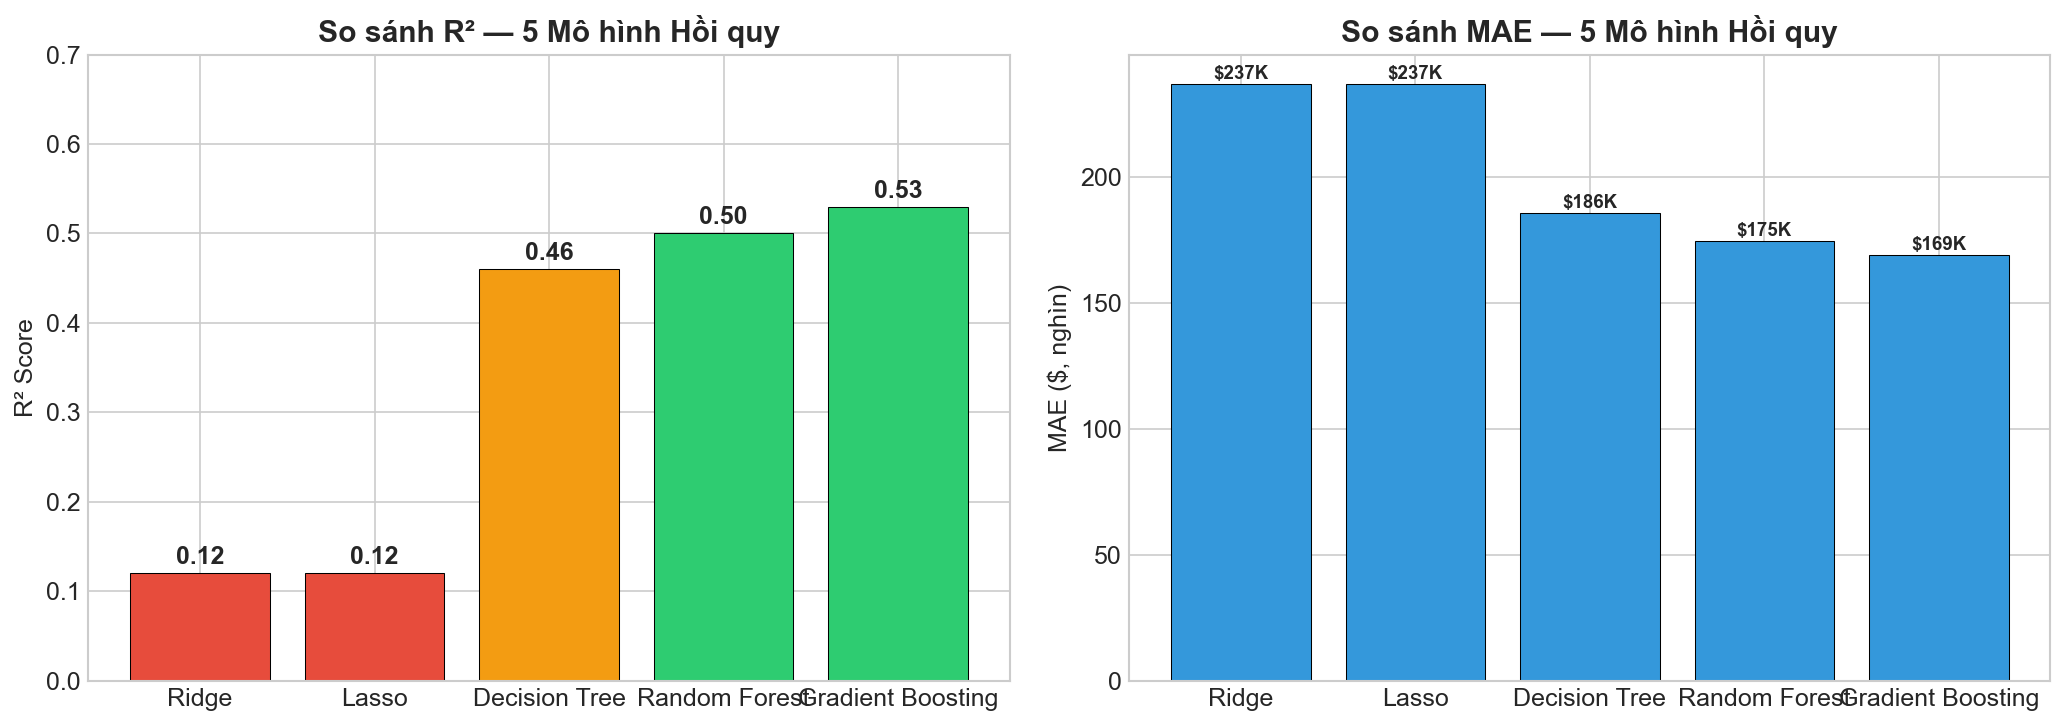
\includegraphics[width=\textwidth]{app2_model_comparison.png}
    \caption{So sánh R² và MAE giữa 5 mô hình hồi quy. Gradient Boosting dẫn đầu nhưng R² = 0.53 cho thấy chỉ giải thích được 53\% phương sai giá — hạn chế do thiếu đặc trưng vị trí chi tiết.}
    \label{fig:app2_models}
\end{figure}

\textbf{Mô hình được chọn}: \textbf{Gradient Boosting} — R² = 0.53 trên Validation, R² = 0.56 trên Test. MAE = \$168,241 có nghĩa trung bình sai lệch khoảng 168 ngàn USD. Giá trị R² tương đối thấp vì dataset chỉ chứa đặc trưng vật lý (bed, bath, size) mà không có đặc trưng vị trí chi tiết (khu phố, trường học, giao thông).

\textbf{Giải thích metric}: $R^2 = 1 - \frac{SS_{res}}{SS_{tot}} = 0.53$ có nghĩa mô hình giải thích 53\% biến thiên giá nhà. $MAE = \$168{,}241$ có nghĩa khi dự đoán giá một căn nhà, trung bình sẽ sai lệch khoảng $\pm$\$168K so với giá thực.

\subsection{Ứng dụng 3: CSAT — 6 Mô hình Phân loại + NLP}

\begin{table}[H]
\centering
\caption{Kết quả 6 mô hình — CSAT (Validation Set)}
\label{tab:app3_models}
\small
\begin{tabular}{|l|l|c|c|c|c|c|}
\hline
\textbf{\#} & \textbf{Mô hình} & \textbf{Dữ liệu} & \textbf{Accuracy} & \textbf{F1} & \textbf{ROC-AUC} & \textbf{Time} \\
\hline
1 & Logistic Regression & Tabular & 0.6369 & 0.7550 & 0.6018 & 5.08s \\
\hline
2 & Decision Tree & Tabular & 0.6724 & 0.7774 & 0.6810 & 1.58s \\
\hline
3 & Random Forest & Tabular & 0.6713 & 0.7756 & 0.6896 & 9.73s \\
\hline
4 & SVM (LinearSVC) & Tabular & 0.6334 & 0.7519 & 0.6004 & 0.65s \\
\hline
5 & \textbf{LR (Text-only)} & \textbf{TF-IDF} & \textbf{0.8378} & \textbf{0.9059} & 0.6905 & 0.45s \\
\hline
6 & LR (Combined) & Tab+Text & 0.7833 & 0.8663 & \textbf{0.7333} & 3.43s \\
\hline
\end{tabular}
\end{table}

\begin{figure}[H]
    \centering
    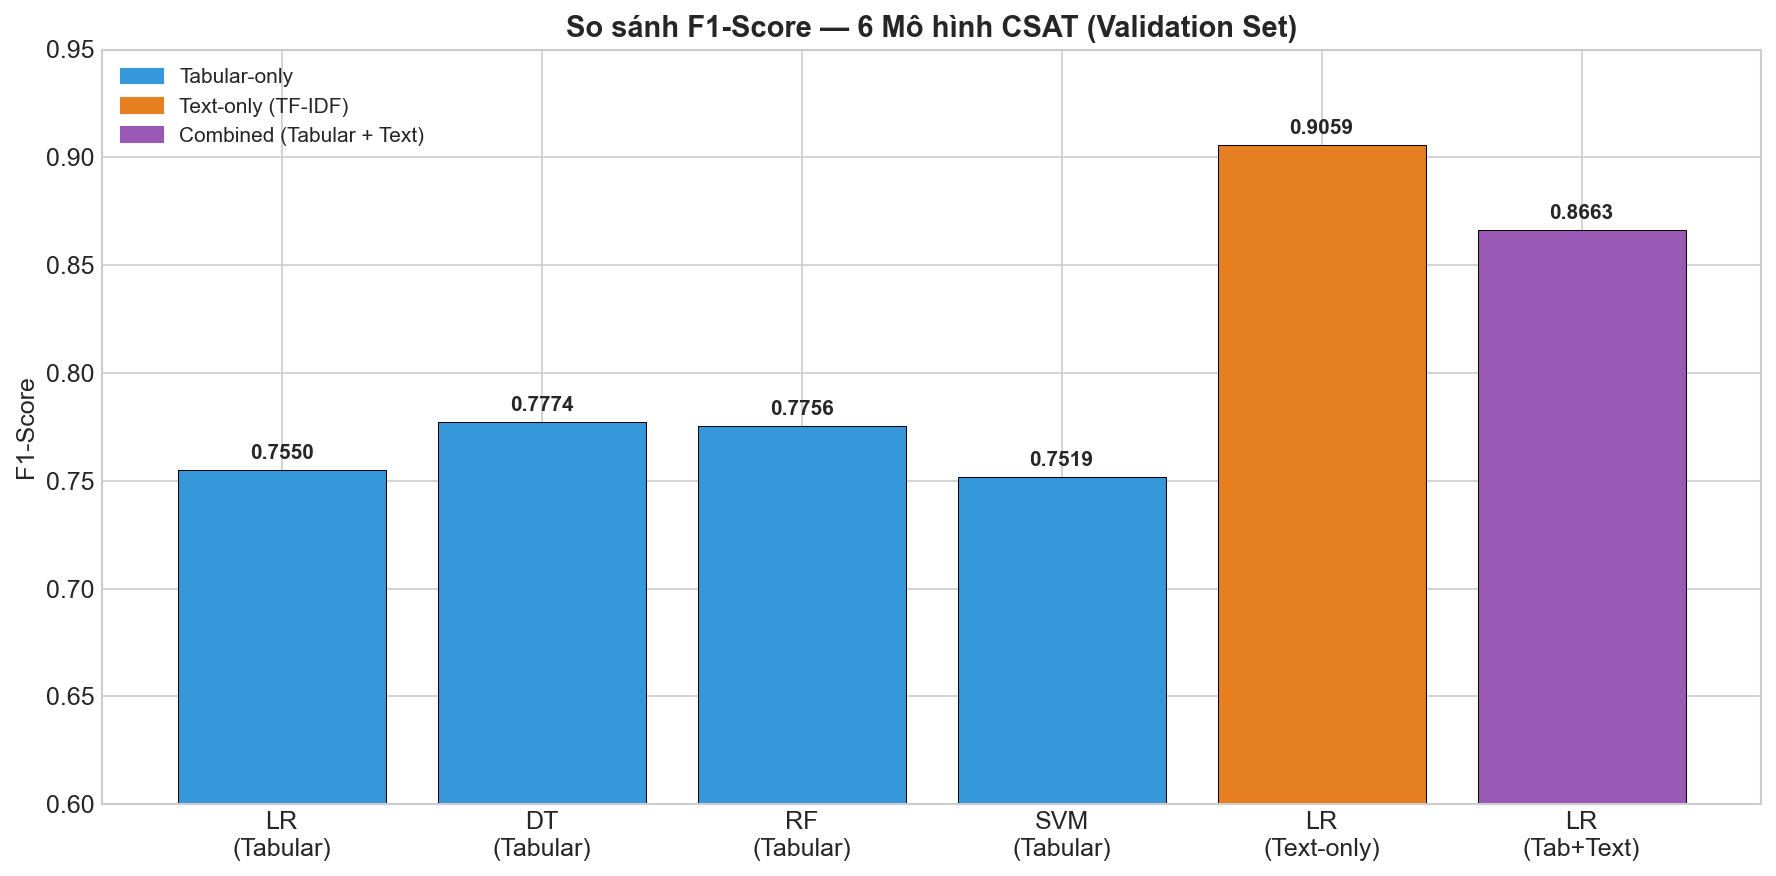
\includegraphics[width=\textwidth]{app3_model_comparison.png}
    \caption{So sánh F1-Score 6 mô hình CSAT. Mô hình Text-only (TF-IDF) đạt F1 cao nhất (0.9059), vượt trội so với mọi mô hình Tabular-only.}
    \label{fig:app3_models}
\end{figure}

\textbf{Phân tích kết quả đáng chú ý}: Mô hình 5 (Text-only) đạt F1 = 0.9059, vượt trội so với mô hình 6 (Combined, F1 = 0.8663). Nguyên nhân:
\begin{itemize}
    \item 66.5\% mẫu \textit{không có} nhận xét (chuỗi rỗng). Với những mẫu này, vector TF-IDF toàn số 0, tạo ra phân phối rõ ràng: ``có text'' vs ``không text''.
    \item Mẫu \textit{có nhận xét} chứa tín hiệu cảm xúc cực kỳ mạnh (``worst'', ``terrible'', ``excellent'') — mô hình tuyến tính dễ dàng phân tách.
    \item Khi kết hợp Tabular, các biến vận hành (thời gian phản hồi, kênh, ca trực) có tương quan yếu hơn với mục tiêu → thêm \textit{nhiễu} khiến F1 giảm nhẹ.
    \item Tuy nhiên, mô hình 6 (Combined) có \textbf{ROC-AUC cao nhất} (0.7333) → cho thấy khả năng phân biệt tổng thể tốt hơn, đặc biệt quan trọng khi thay đổi ngưỡng quyết định.
\end{itemize}

\textbf{Mô hình triển khai}: Mô hình 6 (Combined) được chọn triển khai vì trong thực tế, hệ thống cần hoạt động ngay cả khi khách hàng không để lại nhận xét — lúc này các biến vận hành đóng vai trò ``lá chắn nền tảng''.

% ═══════════════════════════════════════════════════════════
% CHƯƠNG 7: ĐÁNH GIÁ VÀ SO SÁNH
% ═══════════════════════════════════════════════════════════
\section{Đánh giá và So sánh Mô hình}

\subsection{Đánh giá trên tập Test — App1: Diabetes}

Mô hình Gradient Boosting trên tập Test:
\begin{itemize}
    \item Accuracy: 0.9460, Precision: 0.78, Recall: 0.71, F1: 0.7430
    \item ROC-AUC: 0.9510
\end{itemize}

\textbf{Giải thích Confusion Matrix}: Recall = 0.71 nghĩa là 71\% bệnh nhân thực sự mắc tiểu đường được phát hiện đúng. 29\% còn lại bị bỏ sót (False Negative) — trong y tế, đây là chỉ số cần ưu tiên cải thiện vì việc bỏ sót bệnh nhân nguy hiểm hơn việc cảnh báo nhầm.

\subsection{Đánh giá trên tập Test — App2: House Price}

Mô hình Gradient Boosting trên tập Test:
\begin{itemize}
    \item R² = 0.5574, MAE = \$168,241, RMSE = \$337,528, MAPE = 38.2\%
\end{itemize}

\textbf{Giải thích thực tiễn}: Với một căn nhà giá \$400,000, mô hình dự đoán trung bình sai lệch $\pm$\$168K (có thể từ \$232K đến \$568K). MAPE = 38.2\% nghĩa là sai số trung bình 38\% giá trị thực — mức này chấp nhận được cho ước lượng sơ bộ nhưng chưa đủ tin cậy cho giao dịch thực tế.

\subsection{Đánh giá trên tập Test — App3: CSAT}

Mô hình Text-only LR (F1 cao nhất trên Val) trên tập Test:
\begin{itemize}
    \item Accuracy: 0.8378, Precision: 0.8744, Recall: 0.9399, F1: 0.9059
    \item ROC-AUC: 0.6905
\end{itemize}

\textbf{So sánh Tabular vs Text vs Combined}:
\begin{itemize}
    \item \textbf{Tabular-only} (F1 $\sim$ 0.75--0.78): Chỉ dựa vào dữ liệu vận hành, hiệu quả trung bình.
    \item \textbf{Text-only} (F1 = 0.91): Tín hiệu cảm xúc từ nhận xét văn bản mạnh hơn đáng kể.
    \item \textbf{Combined} (F1 = 0.87, ROC-AUC = 0.73): Cân bằng tốt nhất, hoạt động được cả khi có/không text.
\end{itemize}

\subsection{Metric phù hợp nhất cho mỗi ứng dụng}

\begin{itemize}
    \item \textbf{App1 (Diabetes)}: \textbf{Recall} — ưu tiên phát hiện đúng bệnh nhân mắc bệnh (giảm False Negative).
    \item \textbf{App2 (House Price)}: \textbf{MAE + R²} — MAE cho biết sai số tuyệt đối bằng USD, R² cho biết tỷ lệ phương sai giải thích được.
    \item \textbf{App3 (CSAT)}: \textbf{F1-Score} — cân bằng Precision và Recall trong bối cảnh mất cân bằng lớp.
\end{itemize}

% ═══════════════════════════════════════════════════════════
% CHƯƠNG 8: TRIỂN KHAI WEB VÀ MOBILE
% ═══════════════════════════════════════════════════════════
\section{Triển khai Web và Mobile}

\subsection{Kiến trúc triển khai chung}

Cả ba ứng dụng đều tuân theo kiến trúc hai lớp:
\begin{enumerate}
    \item \textbf{REST API (Flask)}: Cung cấp endpoint chuẩn \texttt{POST /predict} cho tích hợp hệ thống.
    \item \textbf{Web UI (FastAPI + Bootstrap 5)}: Giao diện người dùng responsive, hỗ trợ truy cập từ cả desktop và mobile browser.
\end{enumerate}

Quy trình inference: $\text{Raw User Input} \to \text{Validation} \to \text{Same Preprocessing} \to \text{Saved Model} \to \text{Prediction}$.

\textbf{Lưu ý quan trọng}: Preprocessing sử dụng trong triển khai \textit{đúng là pipeline đã \texttt{fit()} trên tập Train}, được nạp lại từ file \texttt{.joblib}. Không có bất kỳ \texttt{fit()} mới nào trên dữ liệu người dùng.

\subsection{Chi tiết triển khai từng ứng dụng}

\begin{table}[H]
\centering
\caption{Thông tin triển khai web cho 3 ứng dụng}
\label{tab:deployment}
\small
\begin{tabularx}{\textwidth}{|l|X|X|X|}
\hline
\textbf{Mục} & \textbf{App1: Diabetes} & \textbf{App2: House Price} & \textbf{App3: CSAT} \\
\hline
Web Framework & FastAPI & FastAPI & FastAPI \\
\hline
REST API & Flask (Port 5001) & Flask (Port 5002) & Flask (Port 5003) \\
\hline
Web UI Port & 8001 & 8002 & 8003 \\
\hline
API Endpoint & \texttt{/predict} & \texttt{/predict} & \texttt{/predict}, \texttt{/csat/v1/predict} \\
\hline
Input & 8 chỉ số lâm sàng & 4 đặc trưng nhà & 6 biến vận hành + 1 text \\
\hline
Model File & \texttt{diabetes\_pipeline.joblib} & \texttt{house\_price\_pipeline.joblib} & \texttt{csat\_pipeline.joblib} \\
\hline
Output & Xác suất mắc bệnh (\%) & Giá ước lượng (USD) & Hài lòng / Rủi ro (\%) \\
\hline
\end{tabularx}
\end{table}

\subsection{Giao diện Người dùng và Triển khai Đa nền tảng}

Cả ba ứng dụng web đều sử dụng \textbf{Bootstrap 5} — framework CSS responsive tự động điều chỉnh giao diện theo kích thước màn hình. Nhờ vào hệ thống lưới (Grid system) linh hoạt kết hợp Flexbox, giao diện tự động co giãn tối ưu từ màn hình máy tính để bàn (Desktop) đến thiết bị di động (Smartphone/Tablet). Kiến trúc tích hợp thực tế tuân thủ:

$$\text{User Browser (Desktop/Mobile)} \xrightarrow{\text{JSON / Form}} \text{FastAPI/Flask REST API} \xrightarrow{} \text{Preprocessing Pipeline} \xrightarrow{} \text{Saved ML Model} \xrightarrow{} \text{Prediction Response}$$

\subsubsection{Ứng dụng 1: Giao diện Dự đoán Tiểu đường (App1)}
Giao diện App1 cung cấp biểu mẫu nhập 8 chỉ số lâm sàng được chia thành 3 phân khu trực quan: Thông tin cá nhân, Chỉ số sinh thái, và Tiền sử bệnh lý. Kết quả hiển thị dưới dạng thẻ thông báo màu sắc phân biệt rõ ràng (đỏ cho cảnh báo nguy cơ, xanh cho an toàn) cùng thanh đo tỷ lệ xác suất hai lớp.

\begin{figure}[H]
    \centering
    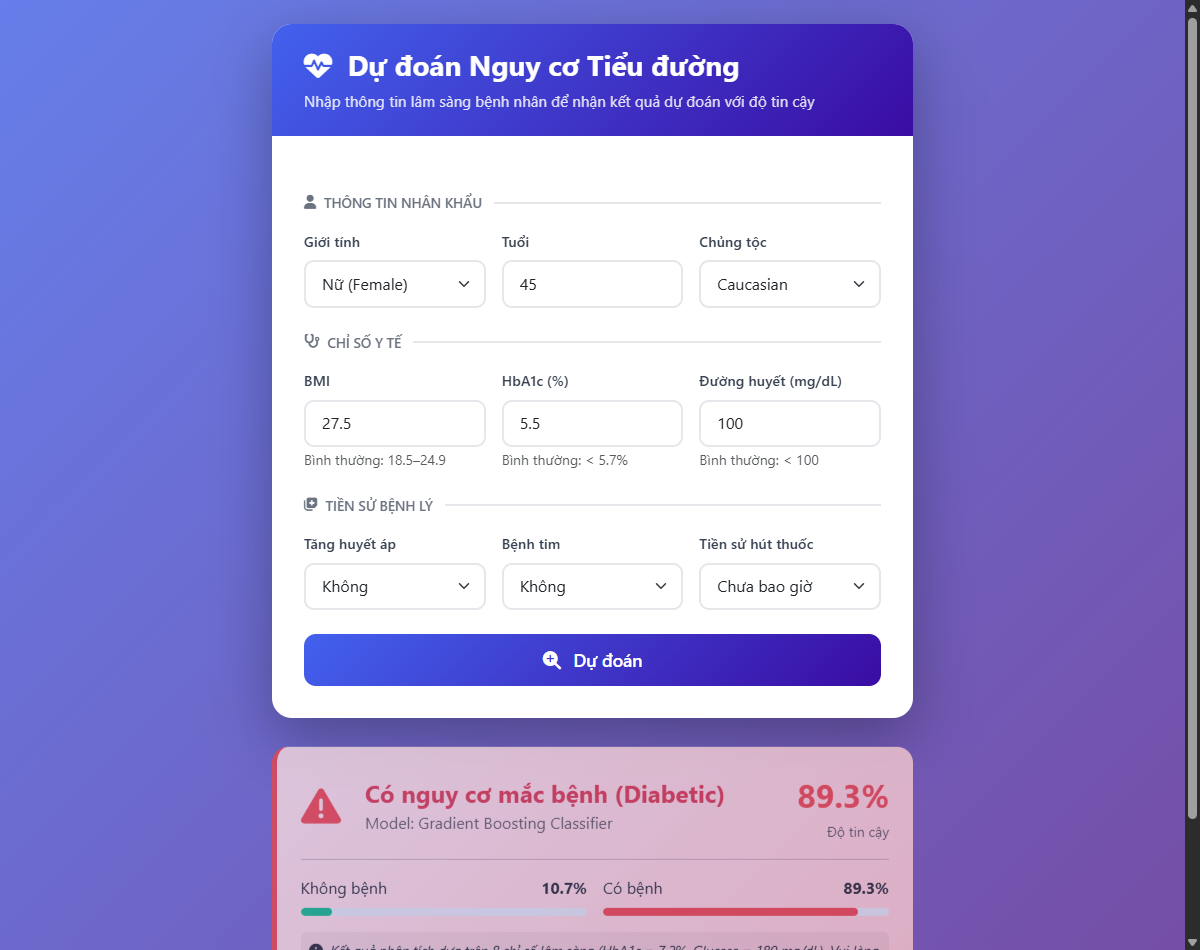
\includegraphics[width=0.85\textwidth]{figures/app1_web_desktop.png}
    \caption{Giao diện Web Desktop của App1 — Dự đoán Bệnh Tiểu đường với kết quả phân tích thời gian thực.}
    \label{fig:app1_desktop}
\end{figure}

\begin{figure}[H]
    \centering
    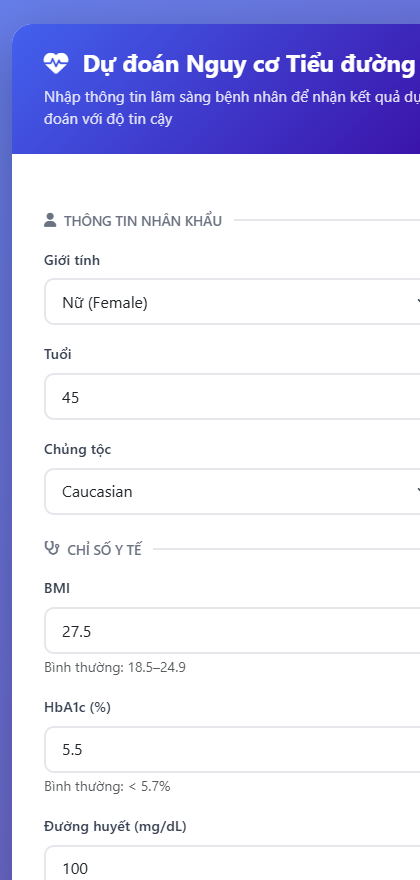
\includegraphics[width=0.42\textwidth]{figures/app1_web_mobile.png}
    \caption{Giao diện Mobile Responsive của App1 trên màn hình điện thoại di động.}
    \label{fig:app1_mobile}
\end{figure}

\subsubsection{Ứng dụng 2: Giao diện Định giá Bất động sản (App2)}
Giao diện App2 cho phép người dùng lựa chọn bang (State dropdown hỗ trợ toàn bộ các bang của Hoa Kỳ), thành phố, tình trạng rao bán và các thuộc tính phòng ở/diện tích. Kết quả hiển thị giá ước tính định dạng tiền tệ USD nổi bật cùng thông tin về sai số và khuyến cáo thị trường.

\begin{figure}[H]
    \centering
    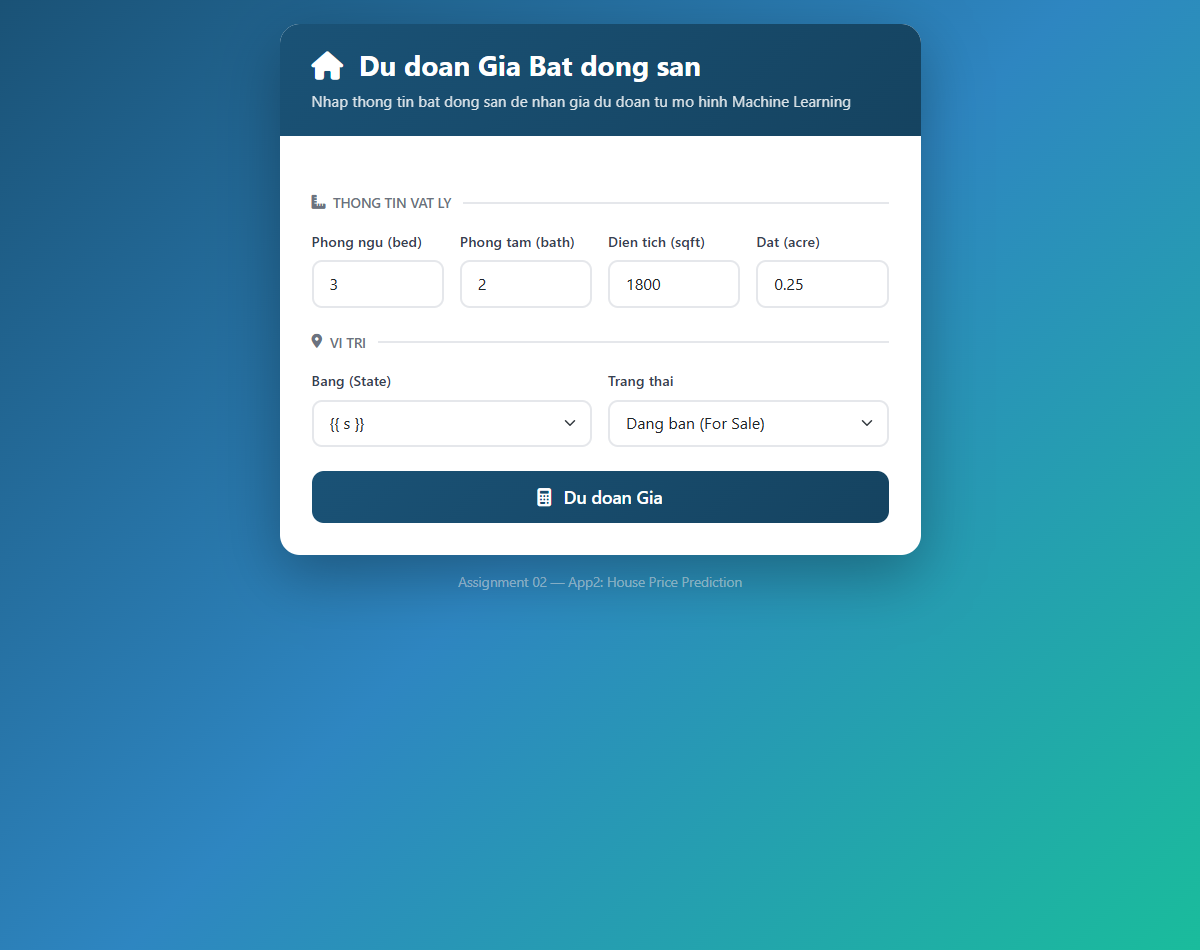
\includegraphics[width=0.85\textwidth]{figures/app2_web_desktop.png}
    \caption{Giao diện Web Desktop của App2 — Định giá Nhà ở Hoa Kỳ.}
    \label{fig:app2_desktop}
\end{figure}

\begin{figure}[H]
    \centering
    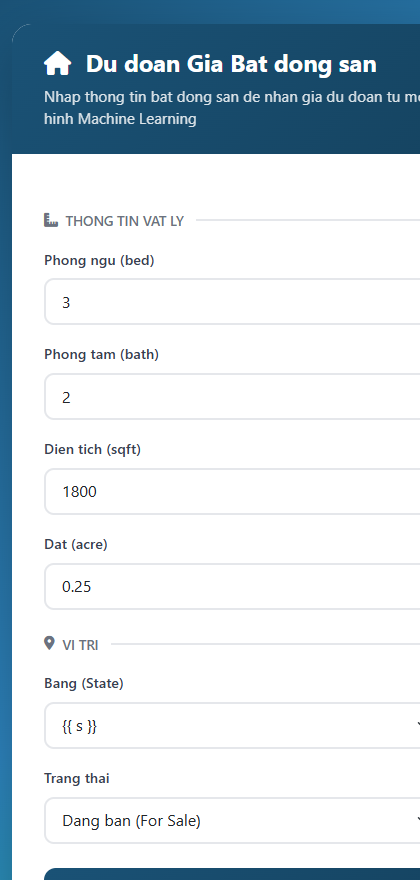
\includegraphics[width=0.42\textwidth]{figures/app2_web_mobile.png}
    \caption{Giao diện Mobile Responsive của App2 trên thiết bị di động.}
    \label{fig:app2_mobile}
\end{figure}

\subsubsection{Ứng dụng 3: Giao diện Dự đoán Mức độ Hài lòng Khách hàng (App3)}
Giao diện App3 nổi bật với khu vực nhập liệu đa phương thức: vừa bao gồm các thông số bảng vận hành (Kênh tiếp nhận, Danh mục sự cố, Thâm niên tư vấn viên, Ca trực, Thời gian phản hồi) vừa có khung văn bản mở (Customer Remarks) cho nhận xét của khách hàng. Mô hình Combined xử lý TF-IDF tức thì và trả về biểu tượng cảm xúc trực quan cùng phần trăm độ tin cậy.

\begin{figure}[H]
    \centering
    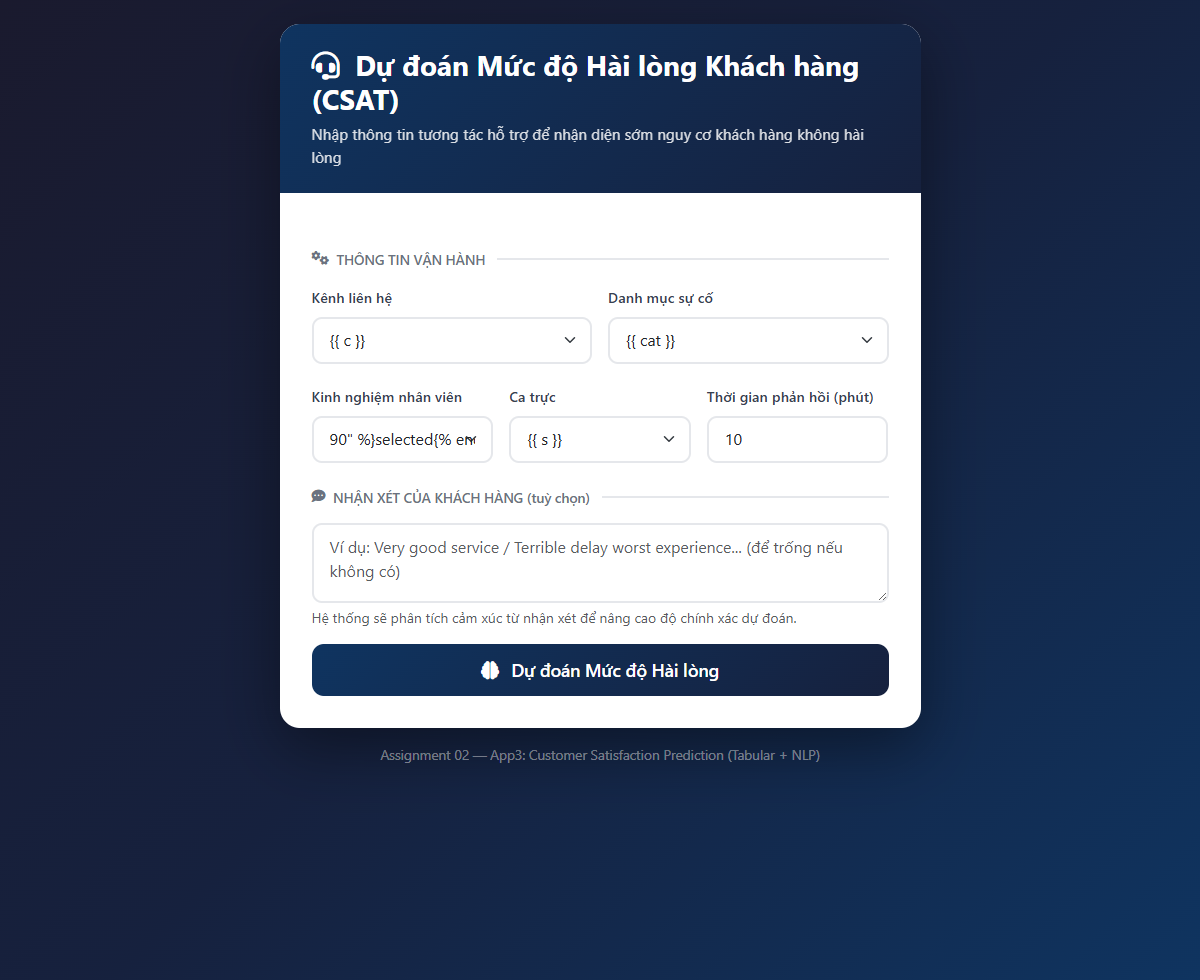
\includegraphics[width=0.85\textwidth]{figures/app3_web_desktop.png}
    \caption{Giao diện Web Desktop của App3 — Đánh giá CSAT kết hợp phân tích văn bản NLP.}
    \label{fig:app3_desktop}
\end{figure}

\begin{figure}[H]
    \centering
    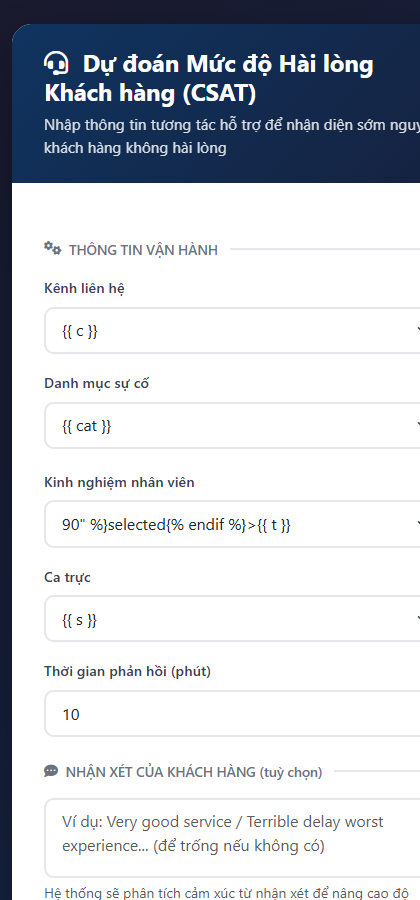
\includegraphics[width=0.42\textwidth]{figures/app3_web_mobile.png}
    \caption{Giao diện Mobile Responsive của App3 trên màn hình điện thoại di động.}
    \label{fig:app3_mobile}
\end{figure}

\subsection{Ví dụ Request/Response}

\textbf{App1 — Diabetes Prediction:}
\begin{lstlisting}
# Request
POST http://localhost:5001/diabetes/v1/predict
{
    "gender": "Female", "age": 55, "bmi": 32.5,
    "hba1c": 7.2, "blood_glucose": 180,
    "hypertension": 1, "heart_disease": 0,
    "smoking": "current"
}

# Response
{
    "prediction": 1,
    "label": "Diabetic",
    "confidence": 89.3,
    "probability_diabetic": 89.3
}
\end{lstlisting}

\textbf{App3 — CSAT Prediction (có nhận xét văn bản):}
\begin{lstlisting}
# Request
POST http://localhost:5003/csat/v1/predict
{
    "channel": "Email", "category": "Refund Related",
    "tenure": "On Job Training", "shift": "Night",
    "response_time": 200,
    "remarks": "Terrible delay worst experience"
}

# Response
{
    "prediction": 0,
    "label": "At-Risk",
    "confidence": 97.2,
    "probability_at_risk": 97.2
}
\end{lstlisting}

% ═══════════════════════════════════════════════════════════
% CHƯƠNG 9: THẢO LUẬN
% ═══════════════════════════════════════════════════════════
\section{Thảo luận}

\subsection{Bảng So sánh Liên ứng dụng (Cross-Application Comparison)}

\begin{table}[H]
\centering
\caption{Bảng so sánh tổng hợp 3 hệ thống thông minh}
\label{tab:cross_comparison}
\small
\begin{tabularx}{\textwidth}{|l|X|X|X|}
\hline
\textbf{Khía cạnh} & \textbf{Diabetes} & \textbf{House Price} & \textbf{CSAT} \\
\hline
Loại bài toán & Phân loại nhị phân & Hồi quy & Phân loại nhị phân + NLP \\
\hline
1 Observation & Một bệnh nhân & Một căn nhà & Một tương tác CSKH \\
\hline
Biến mục tiêu & \texttt{diabetes} (0/1) & \texttt{price} (USD) & \texttt{is\_satisfied} (0/1) \\
\hline
Kích thước input & $B \times 8$ & $B \times 5$ & $B \times 508$ \\
\hline
Vấn đề chất lượng & Missing gender 17.7\% & price=0, size=0 & 6 cột $>$ 60\% thiếu \\
\hline
Mô hình tốt nhất & Gradient Boosting & Gradient Boosting & LR (Text-only) \\
\hline
Metric chính & F1 = 0.743 & R² = 0.557 & F1 = 0.906 \\
\hline
Web deployment & FastAPI (8001) & FastAPI (8002) & FastAPI (8003) \\
\hline
Mobile & Bootstrap 5 Responsive & Bootstrap 5 Responsive & Bootstrap 5 Responsive \\
\hline
Hạn chế chính & HbA1c chi phối quá mạnh & R² thấp do thiếu vị trí & 66.5\% thiếu text \\
\hline
\end{tabularx}
\end{table}

\subsection{Trả lời 18 Câu hỏi Bắt buộc}

\begin{enumerate}
    \item \textbf{Ba tập dữ liệu khác nhau như thế nào?} \\
    App1 là dữ liệu y tế (chỉ số lâm sàng), App2 là dữ liệu bất động sản (đặc trưng vật lý), App3 là dữ liệu vận hành dịch vụ (tabular + text). Chúng khác nhau về domain, kích thước, loại biến và mức độ phức tạp xử lý.

    \item \textbf{Một observation đại diện cho gì?} \\
    App1: Một bệnh nhân. App2: Một căn nhà rao bán. App3: Một lượt tương tác hỗ trợ khách hàng.

    \item \textbf{Biến mục tiêu của mỗi ứng dụng?} \\
    App1: \texttt{diabetes} (0/1). App2: \texttt{price} (USD). App3: \texttt{is\_satisfied} (0/1).

    \item \textbf{Biểu diễn tính toán?} \\
    App1: Ma trận $B \times 8$. App2: Ma trận $B \times 5$ với target log-transformed. App3: Ma trận thưa $B \times 508$ kết hợp tabular + TF-IDF.

    \item \textbf{Ứng dụng nào dùng classification?} \\
    App1 (Diabetes) và App3 (CSAT).

    \item \textbf{Ứng dụng nào dùng regression?} \\
    App2 (House Price).

    \item \textbf{Biến phân loại được biểu diễn như thế nào?} \\
    Label Encoding (App1: gender, smoking), Ordinal Encoding (App3: tenure), Frequency Encoding (App3: sub-category), Mapping thủ công (App3: channel, shift).

    \item \textbf{Biến số được biểu diễn và chuẩn hóa thế nào?} \\
    StandardScaler cho cả 3 ứng dụng, chỉ fit trên Train set. App2 thêm Log Transform cho target.

    \item \textbf{Vấn đề chất lượng dữ liệu?} \\
    App1: Missing gender, BMI=0. App2: price=0, size=0, phân phối lệch. App3: 6 cột thiếu >60\%, 66.5\% thiếu text.

    \item \textbf{Thao tác tiền xử lý nào cần thiết?} \\
    Chung: Drop NaN, Encoding, StandardScaler, Train/Val/Test split. Riêng App2: Log transform. Riêng App3: TF-IDF vectorization, Feature engineering (response time).

    \item \textbf{Mô hình nào tốt nhất cho mỗi ứng dụng?} \\
    App1: Gradient Boosting (F1=0.743). App2: Gradient Boosting (R²=0.557). App3: LR Text-only (F1=0.906), triển khai Combined (ROC-AUC=0.733).

    \item \textbf{Metric nào phù hợp nhất?} \\
    App1: Recall (y tế — không bỏ sót bệnh). App2: MAE + R² (đo sai số bằng USD). App3: F1-Score (cân bằng trong bối cảnh mất cân bằng lớp).

    \item \textbf{Mô hình tốt nhất có đặc tính triển khai tốt nhất?} \\
    App1 \& App2: Gradient Boosting — tốc độ inference nhanh, kích thước model vừa phải. App3: Mô hình Text-only F1 cao nhất nhưng triển khai Combined vì cần hoạt động khi không có text.

    \item \textbf{Ứng dụng nào dễ triển khai nhất?} \\
    App1 (Diabetes): Input đơn giản (8 số), không cần xử lý text, model nhẹ.

    \item \textbf{Ứng dụng nào khó triển khai nhất?} \\
    App3 (CSAT): Cần xử lý text realtime (TF-IDF transform), kết hợp sparse matrix, nhiều biến cần mapping.

    \item \textbf{Các dạng rò rỉ dữ liệu đã xem xét?} \\
    (a) Không fit scaler/encoder trên test/val set. (b) Không fit TF-IDF trên test set. (c) Không sử dụng biến target trong feature engineering. (d) Pipeline triển khai load chính xác preprocessor từ training.

    \item \textbf{Hạn chế còn lại?} \\
    App1: HbA1c và blood glucose chi phối quá mạnh, có thể gây bias. App2: R² = 0.53 thấp do thiếu vị trí chi tiết. App3: 66.5\% mẫu thiếu text, chỉ có TF-IDF (chưa dùng BERT/Embedding).

    \item \textbf{Cải tiến nếu có thêm thời gian?} \\
    (a) App2: Thêm geospatial features (lat/lon, khoảng cách trường học). (b) App3: Thay TF-IDF bằng Sentence-BERT embeddings. (c) Cả 3: Thêm ứng dụng mobile native (Flutter). (d) Monitoring \& A/B testing trong production.
\end{enumerate}

% ═══════════════════════════════════════════════════════════
% CHƯƠNG 10: KẾT LUẬN
% ═══════════════════════════════════════════════════════════
\section{Kết luận}

Báo cáo đã trình bày quá trình phát triển end-to-end ba hệ thống thông minh, từ dữ liệu thô đến giao diện người dùng có thể sử dụng thực tế:

$$\text{Dữ liệu thô} \to \text{Làm sạch} \to \text{Biểu diễn} \to \text{Học} \to \text{Đánh giá} \to \text{Lưu trữ} \to \text{Triển khai}$$

\subsection{Bài học chính}

Một hệ thống thông minh \textit{không đơn thuần chỉ là một mô hình ML đã huấn luyện}. Nó đòi hỏi sự kết hợp chặt chẽ giữa hiểu biết dữ liệu, thiết kế biểu diễn, đánh giá công bằng, kỹ thuật phần mềm và tư duy người dùng.

\subsection{Thách thức kỹ thuật quan trọng nhất}

\textbf{Chống rò rỉ dữ liệu (Data Leakage)}: Đảm bảo pipeline preprocessing chỉ \texttt{fit()} trên Train và được lưu trữ/nạp lại đúng cách trong deployment. Bất kỳ sai sót nào ở bước này đều dẫn đến kết quả đánh giá lạc quan giả tạo.

\subsection{Vấn đề biểu diễn dữ liệu quan trọng nhất}

\textbf{App3 — Kết hợp Tabular + Text}: Việc chuyển đổi nhận xét văn bản phi cấu trúc thành vector số (TF-IDF) và hợp nhất với đặc trưng bảng (sparse matrix) là bước biểu diễn phức tạp nhất, đòi hỏi cân nhắc kỹ giữa kích thước từ vựng, ngưỡng tần suất và chiến lược xử lý missing text.

\subsection{Bài học ML quan trọng nhất}

\textbf{Không có mô hình ``tốt nhất'' phổ quát}. Gradient Boosting chiến thắng ở App1 và App2 (dữ liệu tabular thuần), nhưng ở App3, một Logistic Regression đơn giản trên TF-IDF lại vượt trội. Điều này khẳng định: \textit{chất lượng biểu diễn dữ liệu quan trọng hơn độ phức tạp thuật toán}.

\subsection{Bài học triển khai quan trọng nhất}

Việc đóng gói \texttt{model + preprocessor + metadata} thành một artifact duy nhất (\texttt{.joblib}) và nạp lại trong API giúp đảm bảo tính nhất quán giữa training và inference. Kiến trúc \texttt{FastAPI + Flask REST API} cho phép tách biệt giao diện (frontend) khỏi logic dự đoán (backend).

\subsection{Đề xuất cải tiến tương lai}

\begin{enumerate}
    \item Thêm geospatial features cho App2 (latitude, longitude, khoảng cách tiện ích).
    \item Thay TF-IDF bằng Sentence-BERT embeddings cho App3 để nắm bắt ngữ nghĩa sâu hơn.
    \item Xây dựng ứng dụng mobile native bằng Flutter kết nối REST API.
    \item Thiết lập CI/CD pipeline và model monitoring trong production.
\end{enumerate}

% ═══════════════════════════════════════════════════════════
% PHỤ LỤC: REPRODUCIBILITY
% ═══════════════════════════════════════════════════════════
\newpage
\section*{Phụ lục: Thông tin Tái tạo (Reproducibility)}
\addcontentsline{toc}{section}{Phụ lục: Thông tin Tái tạo}

\begin{table}[H]
\centering
\caption{Thông tin môi trường và tái tạo thí nghiệm}
\label{tab:reproducibility}
\small
\begin{tabularx}{\textwidth}{|l|X|}
\hline
\textbf{Mục} & \textbf{Chi tiết} \\
\hline
Python version & 3.11+ \\
\hline
Hệ điều hành & Windows 10/11 \\
\hline
Random seed & 42 \\
\hline
Thư viện chính & scikit-learn, pandas, numpy, matplotlib, seaborn, scipy \\
\hline
Web frameworks & FastAPI, Flask, Jinja2, Bootstrap 5 \\
\hline
Train/Val/Test split & 70\% / 15\% / 15\% (stratified, random\_state=42) \\
\hline
Preprocessing & \texttt{fit()} chỉ trên Train set, lưu \texttt{.joblib} \\
\hline
\end{tabularx}
\end{table}

\textbf{Hướng dẫn chạy lại}:
\begin{lstlisting}[language=bash]
# 1. Cai dat thu vien
pip install -r requirements.txt

# 2. Chay notebook de huan luyen
jupyter notebook diabetes_classification.ipynb

# 3. Khoi dong REST API
python REST_API.py

# 4. Khoi dong Web UI
uvicorn app:app --reload --port 8001
\end{lstlisting}

\end{document}
